
% Default to the notebook output style

    


% Inherit from the specified cell style.




    
\documentclass[11pt]{article}

    
    
    \usepackage[T1]{fontenc}
    % Nicer default font (+ math font) than Computer Modern for most use cases
    \usepackage{mathpazo}

    % Basic figure setup, for now with no caption control since it's done
    % automatically by Pandoc (which extracts ![](path) syntax from Markdown).
    \usepackage{graphicx}
    % We will generate all images so they have a width \maxwidth. This means
    % that they will get their normal width if they fit onto the page, but
    % are scaled down if they would overflow the margins.
    \makeatletter
    \def\maxwidth{\ifdim\Gin@nat@width>\linewidth\linewidth
    \else\Gin@nat@width\fi}
    \makeatother
    \let\Oldincludegraphics\includegraphics
    % Set max figure width to be 80% of text width, for now hardcoded.
    \renewcommand{\includegraphics}[1]{\Oldincludegraphics[width=.8\maxwidth]{#1}}
    % Ensure that by default, figures have no caption (until we provide a
    % proper Figure object with a Caption API and a way to capture that
    % in the conversion process - todo).
    \usepackage{caption}
    \DeclareCaptionLabelFormat{nolabel}{}
    \captionsetup{labelformat=nolabel}

    \usepackage{adjustbox} % Used to constrain images to a maximum size 
    \usepackage{xcolor} % Allow colors to be defined
    \usepackage{enumerate} % Needed for markdown enumerations to work
    \usepackage{geometry} % Used to adjust the document margins
    \usepackage{amsmath} % Equations
    \usepackage{amssymb} % Equations
    \usepackage{textcomp} % defines textquotesingle
    % Hack from http://tex.stackexchange.com/a/47451/13684:
    \AtBeginDocument{%
        \def\PYZsq{\textquotesingle}% Upright quotes in Pygmentized code
    }
    \usepackage{upquote} % Upright quotes for verbatim code
    \usepackage{eurosym} % defines \euro
    \usepackage[mathletters]{ucs} % Extended unicode (utf-8) support
    \usepackage[utf8x]{inputenc} % Allow utf-8 characters in the tex document
    \usepackage{fancyvrb} % verbatim replacement that allows latex
    \usepackage{grffile} % extends the file name processing of package graphics 
                         % to support a larger range 
    % The hyperref package gives us a pdf with properly built
    % internal navigation ('pdf bookmarks' for the table of contents,
    % internal cross-reference links, web links for URLs, etc.)
    \usepackage{hyperref}
    \usepackage{longtable} % longtable support required by pandoc >1.10
    \usepackage{booktabs}  % table support for pandoc > 1.12.2
    \usepackage[inline]{enumitem} % IRkernel/repr support (it uses the enumerate* environment)
    \usepackage[normalem]{ulem} % ulem is needed to support strikethroughs (\sout)
                                % normalem makes italics be italics, not underlines
    

    
    
    % Colors for the hyperref package
    \definecolor{urlcolor}{rgb}{0,.145,.698}
    \definecolor{linkcolor}{rgb}{.71,0.21,0.01}
    \definecolor{citecolor}{rgb}{.12,.54,.11}

    % ANSI colors
    \definecolor{ansi-black}{HTML}{3E424D}
    \definecolor{ansi-black-intense}{HTML}{282C36}
    \definecolor{ansi-red}{HTML}{E75C58}
    \definecolor{ansi-red-intense}{HTML}{B22B31}
    \definecolor{ansi-green}{HTML}{00A250}
    \definecolor{ansi-green-intense}{HTML}{007427}
    \definecolor{ansi-yellow}{HTML}{DDB62B}
    \definecolor{ansi-yellow-intense}{HTML}{B27D12}
    \definecolor{ansi-blue}{HTML}{208FFB}
    \definecolor{ansi-blue-intense}{HTML}{0065CA}
    \definecolor{ansi-magenta}{HTML}{D160C4}
    \definecolor{ansi-magenta-intense}{HTML}{A03196}
    \definecolor{ansi-cyan}{HTML}{60C6C8}
    \definecolor{ansi-cyan-intense}{HTML}{258F8F}
    \definecolor{ansi-white}{HTML}{C5C1B4}
    \definecolor{ansi-white-intense}{HTML}{A1A6B2}

    % commands and environments needed by pandoc snippets
    % extracted from the output of `pandoc -s`
    \providecommand{\tightlist}{%
      \setlength{\itemsep}{0pt}\setlength{\parskip}{0pt}}
    \DefineVerbatimEnvironment{Highlighting}{Verbatim}{commandchars=\\\{\}}
    % Add ',fontsize=\small' for more characters per line
    \newenvironment{Shaded}{}{}
    \newcommand{\KeywordTok}[1]{\textcolor[rgb]{0.00,0.44,0.13}{\textbf{{#1}}}}
    \newcommand{\DataTypeTok}[1]{\textcolor[rgb]{0.56,0.13,0.00}{{#1}}}
    \newcommand{\DecValTok}[1]{\textcolor[rgb]{0.25,0.63,0.44}{{#1}}}
    \newcommand{\BaseNTok}[1]{\textcolor[rgb]{0.25,0.63,0.44}{{#1}}}
    \newcommand{\FloatTok}[1]{\textcolor[rgb]{0.25,0.63,0.44}{{#1}}}
    \newcommand{\CharTok}[1]{\textcolor[rgb]{0.25,0.44,0.63}{{#1}}}
    \newcommand{\StringTok}[1]{\textcolor[rgb]{0.25,0.44,0.63}{{#1}}}
    \newcommand{\CommentTok}[1]{\textcolor[rgb]{0.38,0.63,0.69}{\textit{{#1}}}}
    \newcommand{\OtherTok}[1]{\textcolor[rgb]{0.00,0.44,0.13}{{#1}}}
    \newcommand{\AlertTok}[1]{\textcolor[rgb]{1.00,0.00,0.00}{\textbf{{#1}}}}
    \newcommand{\FunctionTok}[1]{\textcolor[rgb]{0.02,0.16,0.49}{{#1}}}
    \newcommand{\RegionMarkerTok}[1]{{#1}}
    \newcommand{\ErrorTok}[1]{\textcolor[rgb]{1.00,0.00,0.00}{\textbf{{#1}}}}
    \newcommand{\NormalTok}[1]{{#1}}
    
    % Additional commands for more recent versions of Pandoc
    \newcommand{\ConstantTok}[1]{\textcolor[rgb]{0.53,0.00,0.00}{{#1}}}
    \newcommand{\SpecialCharTok}[1]{\textcolor[rgb]{0.25,0.44,0.63}{{#1}}}
    \newcommand{\VerbatimStringTok}[1]{\textcolor[rgb]{0.25,0.44,0.63}{{#1}}}
    \newcommand{\SpecialStringTok}[1]{\textcolor[rgb]{0.73,0.40,0.53}{{#1}}}
    \newcommand{\ImportTok}[1]{{#1}}
    \newcommand{\DocumentationTok}[1]{\textcolor[rgb]{0.73,0.13,0.13}{\textit{{#1}}}}
    \newcommand{\AnnotationTok}[1]{\textcolor[rgb]{0.38,0.63,0.69}{\textbf{\textit{{#1}}}}}
    \newcommand{\CommentVarTok}[1]{\textcolor[rgb]{0.38,0.63,0.69}{\textbf{\textit{{#1}}}}}
    \newcommand{\VariableTok}[1]{\textcolor[rgb]{0.10,0.09,0.49}{{#1}}}
    \newcommand{\ControlFlowTok}[1]{\textcolor[rgb]{0.00,0.44,0.13}{\textbf{{#1}}}}
    \newcommand{\OperatorTok}[1]{\textcolor[rgb]{0.40,0.40,0.40}{{#1}}}
    \newcommand{\BuiltInTok}[1]{{#1}}
    \newcommand{\ExtensionTok}[1]{{#1}}
    \newcommand{\PreprocessorTok}[1]{\textcolor[rgb]{0.74,0.48,0.00}{{#1}}}
    \newcommand{\AttributeTok}[1]{\textcolor[rgb]{0.49,0.56,0.16}{{#1}}}
    \newcommand{\InformationTok}[1]{\textcolor[rgb]{0.38,0.63,0.69}{\textbf{\textit{{#1}}}}}
    \newcommand{\WarningTok}[1]{\textcolor[rgb]{0.38,0.63,0.69}{\textbf{\textit{{#1}}}}}
    
    
    % Define a nice break command that doesn't care if a line doesn't already
    % exist.
    \def\br{\hspace*{\fill} \\* }
    % Math Jax compatability definitions
    \def\gt{>}
    \def\lt{<}
    % Document parameters
    \title{dog\_app}
    
    
    

    % Pygments definitions
    
\makeatletter
\def\PY@reset{\let\PY@it=\relax \let\PY@bf=\relax%
    \let\PY@ul=\relax \let\PY@tc=\relax%
    \let\PY@bc=\relax \let\PY@ff=\relax}
\def\PY@tok#1{\csname PY@tok@#1\endcsname}
\def\PY@toks#1+{\ifx\relax#1\empty\else%
    \PY@tok{#1}\expandafter\PY@toks\fi}
\def\PY@do#1{\PY@bc{\PY@tc{\PY@ul{%
    \PY@it{\PY@bf{\PY@ff{#1}}}}}}}
\def\PY#1#2{\PY@reset\PY@toks#1+\relax+\PY@do{#2}}

\expandafter\def\csname PY@tok@w\endcsname{\def\PY@tc##1{\textcolor[rgb]{0.73,0.73,0.73}{##1}}}
\expandafter\def\csname PY@tok@c\endcsname{\let\PY@it=\textit\def\PY@tc##1{\textcolor[rgb]{0.25,0.50,0.50}{##1}}}
\expandafter\def\csname PY@tok@cp\endcsname{\def\PY@tc##1{\textcolor[rgb]{0.74,0.48,0.00}{##1}}}
\expandafter\def\csname PY@tok@k\endcsname{\let\PY@bf=\textbf\def\PY@tc##1{\textcolor[rgb]{0.00,0.50,0.00}{##1}}}
\expandafter\def\csname PY@tok@kp\endcsname{\def\PY@tc##1{\textcolor[rgb]{0.00,0.50,0.00}{##1}}}
\expandafter\def\csname PY@tok@kt\endcsname{\def\PY@tc##1{\textcolor[rgb]{0.69,0.00,0.25}{##1}}}
\expandafter\def\csname PY@tok@o\endcsname{\def\PY@tc##1{\textcolor[rgb]{0.40,0.40,0.40}{##1}}}
\expandafter\def\csname PY@tok@ow\endcsname{\let\PY@bf=\textbf\def\PY@tc##1{\textcolor[rgb]{0.67,0.13,1.00}{##1}}}
\expandafter\def\csname PY@tok@nb\endcsname{\def\PY@tc##1{\textcolor[rgb]{0.00,0.50,0.00}{##1}}}
\expandafter\def\csname PY@tok@nf\endcsname{\def\PY@tc##1{\textcolor[rgb]{0.00,0.00,1.00}{##1}}}
\expandafter\def\csname PY@tok@nc\endcsname{\let\PY@bf=\textbf\def\PY@tc##1{\textcolor[rgb]{0.00,0.00,1.00}{##1}}}
\expandafter\def\csname PY@tok@nn\endcsname{\let\PY@bf=\textbf\def\PY@tc##1{\textcolor[rgb]{0.00,0.00,1.00}{##1}}}
\expandafter\def\csname PY@tok@ne\endcsname{\let\PY@bf=\textbf\def\PY@tc##1{\textcolor[rgb]{0.82,0.25,0.23}{##1}}}
\expandafter\def\csname PY@tok@nv\endcsname{\def\PY@tc##1{\textcolor[rgb]{0.10,0.09,0.49}{##1}}}
\expandafter\def\csname PY@tok@no\endcsname{\def\PY@tc##1{\textcolor[rgb]{0.53,0.00,0.00}{##1}}}
\expandafter\def\csname PY@tok@nl\endcsname{\def\PY@tc##1{\textcolor[rgb]{0.63,0.63,0.00}{##1}}}
\expandafter\def\csname PY@tok@ni\endcsname{\let\PY@bf=\textbf\def\PY@tc##1{\textcolor[rgb]{0.60,0.60,0.60}{##1}}}
\expandafter\def\csname PY@tok@na\endcsname{\def\PY@tc##1{\textcolor[rgb]{0.49,0.56,0.16}{##1}}}
\expandafter\def\csname PY@tok@nt\endcsname{\let\PY@bf=\textbf\def\PY@tc##1{\textcolor[rgb]{0.00,0.50,0.00}{##1}}}
\expandafter\def\csname PY@tok@nd\endcsname{\def\PY@tc##1{\textcolor[rgb]{0.67,0.13,1.00}{##1}}}
\expandafter\def\csname PY@tok@s\endcsname{\def\PY@tc##1{\textcolor[rgb]{0.73,0.13,0.13}{##1}}}
\expandafter\def\csname PY@tok@sd\endcsname{\let\PY@it=\textit\def\PY@tc##1{\textcolor[rgb]{0.73,0.13,0.13}{##1}}}
\expandafter\def\csname PY@tok@si\endcsname{\let\PY@bf=\textbf\def\PY@tc##1{\textcolor[rgb]{0.73,0.40,0.53}{##1}}}
\expandafter\def\csname PY@tok@se\endcsname{\let\PY@bf=\textbf\def\PY@tc##1{\textcolor[rgb]{0.73,0.40,0.13}{##1}}}
\expandafter\def\csname PY@tok@sr\endcsname{\def\PY@tc##1{\textcolor[rgb]{0.73,0.40,0.53}{##1}}}
\expandafter\def\csname PY@tok@ss\endcsname{\def\PY@tc##1{\textcolor[rgb]{0.10,0.09,0.49}{##1}}}
\expandafter\def\csname PY@tok@sx\endcsname{\def\PY@tc##1{\textcolor[rgb]{0.00,0.50,0.00}{##1}}}
\expandafter\def\csname PY@tok@m\endcsname{\def\PY@tc##1{\textcolor[rgb]{0.40,0.40,0.40}{##1}}}
\expandafter\def\csname PY@tok@gh\endcsname{\let\PY@bf=\textbf\def\PY@tc##1{\textcolor[rgb]{0.00,0.00,0.50}{##1}}}
\expandafter\def\csname PY@tok@gu\endcsname{\let\PY@bf=\textbf\def\PY@tc##1{\textcolor[rgb]{0.50,0.00,0.50}{##1}}}
\expandafter\def\csname PY@tok@gd\endcsname{\def\PY@tc##1{\textcolor[rgb]{0.63,0.00,0.00}{##1}}}
\expandafter\def\csname PY@tok@gi\endcsname{\def\PY@tc##1{\textcolor[rgb]{0.00,0.63,0.00}{##1}}}
\expandafter\def\csname PY@tok@gr\endcsname{\def\PY@tc##1{\textcolor[rgb]{1.00,0.00,0.00}{##1}}}
\expandafter\def\csname PY@tok@ge\endcsname{\let\PY@it=\textit}
\expandafter\def\csname PY@tok@gs\endcsname{\let\PY@bf=\textbf}
\expandafter\def\csname PY@tok@gp\endcsname{\let\PY@bf=\textbf\def\PY@tc##1{\textcolor[rgb]{0.00,0.00,0.50}{##1}}}
\expandafter\def\csname PY@tok@go\endcsname{\def\PY@tc##1{\textcolor[rgb]{0.53,0.53,0.53}{##1}}}
\expandafter\def\csname PY@tok@gt\endcsname{\def\PY@tc##1{\textcolor[rgb]{0.00,0.27,0.87}{##1}}}
\expandafter\def\csname PY@tok@err\endcsname{\def\PY@bc##1{\setlength{\fboxsep}{0pt}\fcolorbox[rgb]{1.00,0.00,0.00}{1,1,1}{\strut ##1}}}
\expandafter\def\csname PY@tok@kc\endcsname{\let\PY@bf=\textbf\def\PY@tc##1{\textcolor[rgb]{0.00,0.50,0.00}{##1}}}
\expandafter\def\csname PY@tok@kd\endcsname{\let\PY@bf=\textbf\def\PY@tc##1{\textcolor[rgb]{0.00,0.50,0.00}{##1}}}
\expandafter\def\csname PY@tok@kn\endcsname{\let\PY@bf=\textbf\def\PY@tc##1{\textcolor[rgb]{0.00,0.50,0.00}{##1}}}
\expandafter\def\csname PY@tok@kr\endcsname{\let\PY@bf=\textbf\def\PY@tc##1{\textcolor[rgb]{0.00,0.50,0.00}{##1}}}
\expandafter\def\csname PY@tok@bp\endcsname{\def\PY@tc##1{\textcolor[rgb]{0.00,0.50,0.00}{##1}}}
\expandafter\def\csname PY@tok@fm\endcsname{\def\PY@tc##1{\textcolor[rgb]{0.00,0.00,1.00}{##1}}}
\expandafter\def\csname PY@tok@vc\endcsname{\def\PY@tc##1{\textcolor[rgb]{0.10,0.09,0.49}{##1}}}
\expandafter\def\csname PY@tok@vg\endcsname{\def\PY@tc##1{\textcolor[rgb]{0.10,0.09,0.49}{##1}}}
\expandafter\def\csname PY@tok@vi\endcsname{\def\PY@tc##1{\textcolor[rgb]{0.10,0.09,0.49}{##1}}}
\expandafter\def\csname PY@tok@vm\endcsname{\def\PY@tc##1{\textcolor[rgb]{0.10,0.09,0.49}{##1}}}
\expandafter\def\csname PY@tok@sa\endcsname{\def\PY@tc##1{\textcolor[rgb]{0.73,0.13,0.13}{##1}}}
\expandafter\def\csname PY@tok@sb\endcsname{\def\PY@tc##1{\textcolor[rgb]{0.73,0.13,0.13}{##1}}}
\expandafter\def\csname PY@tok@sc\endcsname{\def\PY@tc##1{\textcolor[rgb]{0.73,0.13,0.13}{##1}}}
\expandafter\def\csname PY@tok@dl\endcsname{\def\PY@tc##1{\textcolor[rgb]{0.73,0.13,0.13}{##1}}}
\expandafter\def\csname PY@tok@s2\endcsname{\def\PY@tc##1{\textcolor[rgb]{0.73,0.13,0.13}{##1}}}
\expandafter\def\csname PY@tok@sh\endcsname{\def\PY@tc##1{\textcolor[rgb]{0.73,0.13,0.13}{##1}}}
\expandafter\def\csname PY@tok@s1\endcsname{\def\PY@tc##1{\textcolor[rgb]{0.73,0.13,0.13}{##1}}}
\expandafter\def\csname PY@tok@mb\endcsname{\def\PY@tc##1{\textcolor[rgb]{0.40,0.40,0.40}{##1}}}
\expandafter\def\csname PY@tok@mf\endcsname{\def\PY@tc##1{\textcolor[rgb]{0.40,0.40,0.40}{##1}}}
\expandafter\def\csname PY@tok@mh\endcsname{\def\PY@tc##1{\textcolor[rgb]{0.40,0.40,0.40}{##1}}}
\expandafter\def\csname PY@tok@mi\endcsname{\def\PY@tc##1{\textcolor[rgb]{0.40,0.40,0.40}{##1}}}
\expandafter\def\csname PY@tok@il\endcsname{\def\PY@tc##1{\textcolor[rgb]{0.40,0.40,0.40}{##1}}}
\expandafter\def\csname PY@tok@mo\endcsname{\def\PY@tc##1{\textcolor[rgb]{0.40,0.40,0.40}{##1}}}
\expandafter\def\csname PY@tok@ch\endcsname{\let\PY@it=\textit\def\PY@tc##1{\textcolor[rgb]{0.25,0.50,0.50}{##1}}}
\expandafter\def\csname PY@tok@cm\endcsname{\let\PY@it=\textit\def\PY@tc##1{\textcolor[rgb]{0.25,0.50,0.50}{##1}}}
\expandafter\def\csname PY@tok@cpf\endcsname{\let\PY@it=\textit\def\PY@tc##1{\textcolor[rgb]{0.25,0.50,0.50}{##1}}}
\expandafter\def\csname PY@tok@c1\endcsname{\let\PY@it=\textit\def\PY@tc##1{\textcolor[rgb]{0.25,0.50,0.50}{##1}}}
\expandafter\def\csname PY@tok@cs\endcsname{\let\PY@it=\textit\def\PY@tc##1{\textcolor[rgb]{0.25,0.50,0.50}{##1}}}

\def\PYZbs{\char`\\}
\def\PYZus{\char`\_}
\def\PYZob{\char`\{}
\def\PYZcb{\char`\}}
\def\PYZca{\char`\^}
\def\PYZam{\char`\&}
\def\PYZlt{\char`\<}
\def\PYZgt{\char`\>}
\def\PYZsh{\char`\#}
\def\PYZpc{\char`\%}
\def\PYZdl{\char`\$}
\def\PYZhy{\char`\-}
\def\PYZsq{\char`\'}
\def\PYZdq{\char`\"}
\def\PYZti{\char`\~}
% for compatibility with earlier versions
\def\PYZat{@}
\def\PYZlb{[}
\def\PYZrb{]}
\makeatother


    % Exact colors from NB
    \definecolor{incolor}{rgb}{0.0, 0.0, 0.5}
    \definecolor{outcolor}{rgb}{0.545, 0.0, 0.0}



    
    % Prevent overflowing lines due to hard-to-break entities
    \sloppy 
    % Setup hyperref package
    \hypersetup{
      breaklinks=true,  % so long urls are correctly broken across lines
      colorlinks=true,
      urlcolor=urlcolor,
      linkcolor=linkcolor,
      citecolor=citecolor,
      }
    % Slightly bigger margins than the latex defaults
    
    \geometry{verbose,tmargin=1in,bmargin=1in,lmargin=1in,rmargin=1in}
    
    

    \begin{document}
    
    
    \maketitle
    
    

    
    \hypertarget{convolutional-neural-networks}{%
\section{Convolutional Neural
Networks}\label{convolutional-neural-networks}}

\hypertarget{project-write-an-algorithm-for-a-dog-identification-app}{%
\subsection{Project: Write an Algorithm for a Dog Identification
App}\label{project-write-an-algorithm-for-a-dog-identification-app}}

\begin{center}\rule{0.5\linewidth}{\linethickness}\end{center}

In this notebook, some template code has already been provided for you,
and you will need to implement additional functionality to successfully
complete this project. You will not need to modify the included code
beyond what is requested. Sections that begin with
\textbf{`(IMPLEMENTATION)'} in the header indicate that the following
block of code will require additional functionality which you must
provide. Instructions will be provided for each section, and the
specifics of the implementation are marked in the code block with a
`TODO' statement. Please be sure to read the instructions carefully!

\begin{quote}
\textbf{Note}: Once you have completed all of the code implementations,
you need to finalize your work by exporting the Jupyter Notebook as an
HTML document. Before exporting the notebook to html, all of the code
cells need to have been run so that reviewers can see the final
implementation and output. You can then export the notebook by using the
menu above and navigating to \textbf{File -\textgreater{} Download as
-\textgreater{} HTML (.html)}. Include the finished document along with
this notebook as your submission.
\end{quote}

In addition to implementing code, there will be questions that you must
answer which relate to the project and your implementation. Each section
where you will answer a question is preceded by a \textbf{`Question X'}
header. Carefully read each question and provide thorough answers in the
following text boxes that begin with \textbf{`Answer:'}. Your project
submission will be evaluated based on your answers to each of the
questions and the implementation you provide.

\begin{quote}
\textbf{Note:} Code and Markdown cells can be executed using the
\textbf{Shift + Enter} keyboard shortcut. Markdown cells can be edited
by double-clicking the cell to enter edit mode.
\end{quote}

The rubric contains \emph{optional} ``Stand Out Suggestions'' for
enhancing the project beyond the minimum requirements. If you decide to
pursue the ``Stand Out Suggestions'', you should include the code in
this Jupyter notebook.

 \#\# Step 0: Import Datasets

Make sure that you've downloaded the required human and dog datasets: *
Download the
\href{https://s3-us-west-1.amazonaws.com/udacity-aind/dog-project/dogImages.zip}{dog
dataset}. Unzip the folder and place it in this project's home
directory, at the location \texttt{/dogImages}.

\begin{itemize}
\tightlist
\item
  Download the
  \href{https://s3-us-west-1.amazonaws.com/udacity-aind/dog-project/lfw.zip}{human
  dataset}. Unzip the folder and place it in the home directory, at
  location \texttt{/lfw}.
\end{itemize}

\emph{Note: If you are using a Windows machine, you are encouraged to
use \href{http://www.7-zip.org/}{7zip} to extract the folder.}

In the code cell below, we save the file paths for both the human (LFW)
dataset and dog dataset in the numpy arrays \texttt{human\_files} and
\texttt{dog\_files}.

    \begin{Verbatim}[commandchars=\\\{\}]
{\color{incolor}In [{\color{incolor}1}]:} \PY{k+kn}{import} \PY{n+nn}{numpy} \PY{k}{as} \PY{n+nn}{np}
        \PY{k+kn}{from} \PY{n+nn}{glob} \PY{k}{import} \PY{n}{glob}
        
        \PY{c+c1}{\PYZsh{} load filenames for human and dog images}
        \PY{n}{human\PYZus{}files} \PY{o}{=} \PY{n}{np}\PY{o}{.}\PY{n}{array}\PY{p}{(}\PY{n}{glob}\PY{p}{(}\PY{l+s+s2}{\PYZdq{}}\PY{l+s+s2}{lfw/*/*}\PY{l+s+s2}{\PYZdq{}}\PY{p}{)}\PY{p}{)}
        \PY{n}{dog\PYZus{}files} \PY{o}{=} \PY{n}{np}\PY{o}{.}\PY{n}{array}\PY{p}{(}\PY{n}{glob}\PY{p}{(}\PY{l+s+s2}{\PYZdq{}}\PY{l+s+s2}{dogImages/*/*/*}\PY{l+s+s2}{\PYZdq{}}\PY{p}{)}\PY{p}{)}
        
        \PY{c+c1}{\PYZsh{} print number of images in each dataset}
        \PY{n+nb}{print}\PY{p}{(}\PY{l+s+s1}{\PYZsq{}}\PY{l+s+s1}{There are }\PY{l+s+si}{\PYZpc{}d}\PY{l+s+s1}{ total human images.}\PY{l+s+s1}{\PYZsq{}} \PY{o}{\PYZpc{}} \PY{n+nb}{len}\PY{p}{(}\PY{n}{human\PYZus{}files}\PY{p}{)}\PY{p}{)}
        \PY{n+nb}{print}\PY{p}{(}\PY{l+s+s1}{\PYZsq{}}\PY{l+s+s1}{There are }\PY{l+s+si}{\PYZpc{}d}\PY{l+s+s1}{ total dog images.}\PY{l+s+s1}{\PYZsq{}} \PY{o}{\PYZpc{}} \PY{n+nb}{len}\PY{p}{(}\PY{n}{dog\PYZus{}files}\PY{p}{)}\PY{p}{)}
\end{Verbatim}


    \begin{Verbatim}[commandchars=\\\{\}]
There are 13233 total human images.
There are 8351 total dog images.

    \end{Verbatim}

     \#\# Step 1: Detect Humans

In this section, we use OpenCV's implementation of
\href{http://docs.opencv.org/trunk/d7/d8b/tutorial_py_face_detection.html}{Haar
feature-based cascade classifiers} to detect human faces in images.

OpenCV provides many pre-trained face detectors, stored as XML files on
\href{https://github.com/opencv/opencv/tree/master/data/haarcascades}{github}.
We have downloaded one of these detectors and stored it in the
\texttt{haarcascades} directory. In the next code cell, we demonstrate
how to use this detector to find human faces in a sample image.

    \begin{Verbatim}[commandchars=\\\{\}]
{\color{incolor}In [{\color{incolor}2}]:} \PY{k+kn}{import} \PY{n+nn}{cv2}                
        \PY{k+kn}{import} \PY{n+nn}{matplotlib}\PY{n+nn}{.}\PY{n+nn}{pyplot} \PY{k}{as} \PY{n+nn}{plt}                        
        \PY{o}{\PYZpc{}}\PY{k}{matplotlib} inline                               
        
        \PY{c+c1}{\PYZsh{} extract pre\PYZhy{}trained face detector}
        \PY{n}{face\PYZus{}cascade} \PY{o}{=} \PY{n}{cv2}\PY{o}{.}\PY{n}{CascadeClassifier}\PY{p}{(}\PY{l+s+s1}{\PYZsq{}}\PY{l+s+s1}{haarcascades/haarcascade\PYZus{}frontalface\PYZus{}alt.xml}\PY{l+s+s1}{\PYZsq{}}\PY{p}{)}
        
        \PY{c+c1}{\PYZsh{} load color (BGR) image}
        \PY{n}{img} \PY{o}{=} \PY{n}{cv2}\PY{o}{.}\PY{n}{imread}\PY{p}{(}\PY{n}{human\PYZus{}files}\PY{p}{[}\PY{l+m+mi}{0}\PY{p}{]}\PY{p}{)}
        \PY{c+c1}{\PYZsh{} convert BGR image to grayscale}
        \PY{n}{gray} \PY{o}{=} \PY{n}{cv2}\PY{o}{.}\PY{n}{cvtColor}\PY{p}{(}\PY{n}{img}\PY{p}{,} \PY{n}{cv2}\PY{o}{.}\PY{n}{COLOR\PYZus{}BGR2GRAY}\PY{p}{)}
        
        \PY{c+c1}{\PYZsh{} find faces in image}
        \PY{n}{faces} \PY{o}{=} \PY{n}{face\PYZus{}cascade}\PY{o}{.}\PY{n}{detectMultiScale}\PY{p}{(}\PY{n}{gray}\PY{p}{)}
        
        \PY{c+c1}{\PYZsh{} print number of faces detected in the image}
        \PY{n+nb}{print}\PY{p}{(}\PY{l+s+s1}{\PYZsq{}}\PY{l+s+s1}{Number of faces detected:}\PY{l+s+s1}{\PYZsq{}}\PY{p}{,} \PY{n+nb}{len}\PY{p}{(}\PY{n}{faces}\PY{p}{)}\PY{p}{)}
        
        \PY{c+c1}{\PYZsh{} get bounding box for each detected face}
        \PY{k}{for} \PY{p}{(}\PY{n}{x}\PY{p}{,}\PY{n}{y}\PY{p}{,}\PY{n}{w}\PY{p}{,}\PY{n}{h}\PY{p}{)} \PY{o+ow}{in} \PY{n}{faces}\PY{p}{:}
            \PY{c+c1}{\PYZsh{} add bounding box to color image}
            \PY{n}{cv2}\PY{o}{.}\PY{n}{rectangle}\PY{p}{(}\PY{n}{img}\PY{p}{,}\PY{p}{(}\PY{n}{x}\PY{p}{,}\PY{n}{y}\PY{p}{)}\PY{p}{,}\PY{p}{(}\PY{n}{x}\PY{o}{+}\PY{n}{w}\PY{p}{,}\PY{n}{y}\PY{o}{+}\PY{n}{h}\PY{p}{)}\PY{p}{,}\PY{p}{(}\PY{l+m+mi}{255}\PY{p}{,}\PY{l+m+mi}{0}\PY{p}{,}\PY{l+m+mi}{0}\PY{p}{)}\PY{p}{,}\PY{l+m+mi}{2}\PY{p}{)}
            
        \PY{c+c1}{\PYZsh{} convert BGR image to RGB for plotting}
        \PY{n}{cv\PYZus{}rgb} \PY{o}{=} \PY{n}{cv2}\PY{o}{.}\PY{n}{cvtColor}\PY{p}{(}\PY{n}{img}\PY{p}{,} \PY{n}{cv2}\PY{o}{.}\PY{n}{COLOR\PYZus{}BGR2RGB}\PY{p}{)}
        
        \PY{c+c1}{\PYZsh{} display the image, along with bounding box}
        \PY{n}{plt}\PY{o}{.}\PY{n}{imshow}\PY{p}{(}\PY{n}{cv\PYZus{}rgb}\PY{p}{)}
        \PY{n}{plt}\PY{o}{.}\PY{n}{show}\PY{p}{(}\PY{p}{)}
\end{Verbatim}


    \begin{Verbatim}[commandchars=\\\{\}]
Number of faces detected: 1

    \end{Verbatim}

    \begin{center}
    \adjustimage{max size={0.9\linewidth}{0.9\paperheight}}{output_3_1.png}
    \end{center}
    { \hspace*{\fill} \\}
    
    Before using any of the face detectors, it is standard procedure to
convert the images to grayscale. The \texttt{detectMultiScale} function
executes the classifier stored in \texttt{face\_cascade} and takes the
grayscale image as a parameter.

In the above code, \texttt{faces} is a numpy array of detected faces,
where each row corresponds to a detected face. Each detected face is a
1D array with four entries that specifies the bounding box of the
detected face. The first two entries in the array (extracted in the
above code as \texttt{x} and \texttt{y}) specify the horizontal and
vertical positions of the top left corner of the bounding box. The last
two entries in the array (extracted here as \texttt{w} and \texttt{h})
specify the width and height of the box.

\hypertarget{write-a-human-face-detector}{%
\subsubsection{Write a Human Face
Detector}\label{write-a-human-face-detector}}

We can use this procedure to write a function that returns \texttt{True}
if a human face is detected in an image and \texttt{False} otherwise.
This function, aptly named \texttt{face\_detector}, takes a
string-valued file path to an image as input and appears in the code
block below.

    \begin{Verbatim}[commandchars=\\\{\}]
{\color{incolor}In [{\color{incolor}3}]:} \PY{c+c1}{\PYZsh{} returns \PYZdq{}True\PYZdq{} if face is detected in image stored at img\PYZus{}path}
        \PY{k}{def} \PY{n+nf}{face\PYZus{}detector}\PY{p}{(}\PY{n}{img\PYZus{}path}\PY{p}{)}\PY{p}{:}
            \PY{n}{img} \PY{o}{=} \PY{n}{cv2}\PY{o}{.}\PY{n}{imread}\PY{p}{(}\PY{n}{img\PYZus{}path}\PY{p}{)}
            \PY{n}{gray} \PY{o}{=} \PY{n}{cv2}\PY{o}{.}\PY{n}{cvtColor}\PY{p}{(}\PY{n}{img}\PY{p}{,} \PY{n}{cv2}\PY{o}{.}\PY{n}{COLOR\PYZus{}BGR2GRAY}\PY{p}{)}
            \PY{n}{faces} \PY{o}{=} \PY{n}{face\PYZus{}cascade}\PY{o}{.}\PY{n}{detectMultiScale}\PY{p}{(}\PY{n}{gray}\PY{p}{)}
            \PY{k}{return} \PY{n+nb}{len}\PY{p}{(}\PY{n}{faces}\PY{p}{)} \PY{o}{\PYZgt{}} \PY{l+m+mi}{0}
\end{Verbatim}


    \hypertarget{implementation-assess-the-human-face-detector}{%
\subsubsection{(IMPLEMENTATION) Assess the Human Face
Detector}\label{implementation-assess-the-human-face-detector}}

\textbf{Question 1:} Use the code cell below to test the performance of
the \texttt{face\_detector} function.\\
- What percentage of the first 100 images in \texttt{human\_files} have
a detected human face?\\
- What percentage of the first 100 images in \texttt{dog\_files} have a
detected human face?

Ideally, we would like 100\% of human images with a detected face and
0\% of dog images with a detected face. You will see that our algorithm
falls short of this goal, but still gives acceptable performance. We
extract the file paths for the first 100 images from each of the
datasets and store them in the numpy arrays \texttt{human\_files\_short}
and \texttt{dog\_files\_short}.

    \textbf{Answer:}

    \begin{Verbatim}[commandchars=\\\{\}]
{\color{incolor}In [{\color{incolor}4}]:} \PY{k+kn}{from} \PY{n+nn}{tqdm} \PY{k}{import} \PY{n}{tqdm}
        
        \PY{n}{human\PYZus{}files\PYZus{}short} \PY{o}{=} \PY{n}{human\PYZus{}files}\PY{p}{[}\PY{p}{:}\PY{l+m+mi}{100}\PY{p}{]}
        \PY{n}{dog\PYZus{}files\PYZus{}short} \PY{o}{=} \PY{n}{dog\PYZus{}files}\PY{p}{[}\PY{p}{:}\PY{l+m+mi}{100}\PY{p}{]}
        
        \PY{c+c1}{\PYZsh{}\PYZhy{}\PYZsh{}\PYZhy{}\PYZsh{} Do NOT modify the code above this line. \PYZsh{}\PYZhy{}\PYZsh{}\PYZhy{}\PYZsh{}}
        
        \PY{c+c1}{\PYZsh{}\PYZsh{} TODO: Test the performance of the face\PYZus{}detector algorithm }
        \PY{c+c1}{\PYZsh{}\PYZsh{} on the images in human\PYZus{}files\PYZus{}short and dog\PYZus{}files\PYZus{}short.}
        
        \PY{n}{human\PYZus{}files\PYZus{}face\PYZus{}detections} \PY{o}{=} \PY{n}{np}\PY{o}{.}\PY{n}{sum}\PY{p}{(}\PY{p}{[}\PY{n}{face\PYZus{}detector}\PY{p}{(}\PY{n}{i}\PY{p}{)} \PY{k}{for} \PY{n}{i} \PY{o+ow}{in} \PY{n}{human\PYZus{}files\PYZus{}short}\PY{p}{]}\PY{p}{)}
        \PY{n}{dog\PYZus{}files\PYZus{}face\PYZus{}detections} \PY{o}{=} \PY{n}{np}\PY{o}{.}\PY{n}{sum}\PY{p}{(}\PY{p}{[}\PY{n}{face\PYZus{}detector}\PY{p}{(}\PY{n}{i}\PY{p}{)} \PY{k}{for} \PY{n}{i} \PY{o+ow}{in} \PY{n}{dog\PYZus{}files\PYZus{}short}\PY{p}{]}\PY{p}{)}
        
        \PY{n+nb}{print}\PY{p}{(}\PY{l+s+s2}{\PYZdq{}}\PY{l+s+s2}{The percentage of human faces detected in the human images: }\PY{l+s+si}{\PYZob{}\PYZcb{}}\PY{l+s+s2}{\PYZpc{}}\PY{l+s+s2}{\PYZdq{}}\PY{o}{.}\PY{n}{format}\PY{p}{(}\PY{n}{human\PYZus{}files\PYZus{}face\PYZus{}detections}\PY{p}{)}\PY{p}{)}
        \PY{n+nb}{print}\PY{p}{(}\PY{l+s+s2}{\PYZdq{}}\PY{l+s+s2}{The percentage of human faces detected in the dog images: }\PY{l+s+si}{\PYZob{}\PYZcb{}}\PY{l+s+s2}{\PYZpc{}}\PY{l+s+s2}{\PYZdq{}}\PY{o}{.}\PY{n}{format}\PY{p}{(}\PY{n}{dog\PYZus{}files\PYZus{}face\PYZus{}detections}\PY{p}{)}\PY{p}{)}
\end{Verbatim}


    \begin{Verbatim}[commandchars=\\\{\}]
The percentage of human faces detected in the human images: 96\%
The percentage of human faces detected in the dog images: 18\%

    \end{Verbatim}

    We suggest the face detector from OpenCV as a potential way to detect
human images in your algorithm, but you are free to explore other
approaches, especially approaches that make use of deep learning :).
Please use the code cell below to design and test your own face
detection algorithm. If you decide to pursue this \emph{optional} task,
report performance on \texttt{human\_files\_short} and
\texttt{dog\_files\_short}.

    \begin{Verbatim}[commandchars=\\\{\}]
{\color{incolor}In [{\color{incolor}5}]:} \PY{c+c1}{\PYZsh{}\PYZsh{}\PYZsh{} (Optional) }
        \PY{c+c1}{\PYZsh{}\PYZsh{}\PYZsh{} TODO: Test performance of another face detection algorithm.}
        \PY{c+c1}{\PYZsh{}\PYZsh{}\PYZsh{} Feel free to use as many code cells as needed.}
\end{Verbatim}


    \begin{center}\rule{0.5\linewidth}{\linethickness}\end{center}

 \#\# Step 2: Detect Dogs

In this section, we use a
\href{http://pytorch.org/docs/master/torchvision/models.html}{pre-trained
model} to detect dogs in images.

\hypertarget{obtain-pre-trained-vgg-16-model}{%
\subsubsection{Obtain Pre-trained VGG-16
Model}\label{obtain-pre-trained-vgg-16-model}}

The code cell below downloads the VGG-16 model, along with weights that
have been trained on \href{http://www.image-net.org/}{ImageNet}, a very
large, very popular dataset used for image classification and other
vision tasks. ImageNet contains over 10 million URLs, each linking to an
image containing an object from one of
\href{https://gist.github.com/yrevar/942d3a0ac09ec9e5eb3a}{1000
categories}.

    \begin{Verbatim}[commandchars=\\\{\}]
{\color{incolor}In [{\color{incolor}6}]:} \PY{k+kn}{import} \PY{n+nn}{torch}
        \PY{k+kn}{import} \PY{n+nn}{torchvision}\PY{n+nn}{.}\PY{n+nn}{models} \PY{k}{as} \PY{n+nn}{models}
        
        \PY{c+c1}{\PYZsh{} define VGG16 model}
        \PY{n}{VGG16} \PY{o}{=} \PY{n}{models}\PY{o}{.}\PY{n}{vgg16}\PY{p}{(}\PY{n}{pretrained}\PY{o}{=}\PY{k+kc}{True}\PY{p}{)}
        
        \PY{c+c1}{\PYZsh{} check if CUDA is available}
        \PY{n}{use\PYZus{}cuda} \PY{o}{=} \PY{n}{torch}\PY{o}{.}\PY{n}{cuda}\PY{o}{.}\PY{n}{is\PYZus{}available}\PY{p}{(}\PY{p}{)}
        
        \PY{c+c1}{\PYZsh{} move model to GPU if CUDA is available}
        \PY{k}{if} \PY{n}{use\PYZus{}cuda}\PY{p}{:}
            \PY{n}{VGG16} \PY{o}{=} \PY{n}{VGG16}\PY{o}{.}\PY{n}{cuda}\PY{p}{(}\PY{p}{)}
\end{Verbatim}


    Given an image, this pre-trained VGG-16 model returns a prediction
(derived from the 1000 possible categories in ImageNet) for the object
that is contained in the image.

    \hypertarget{implementation-making-predictions-with-a-pre-trained-model}{%
\subsubsection{(IMPLEMENTATION) Making Predictions with a Pre-trained
Model}\label{implementation-making-predictions-with-a-pre-trained-model}}

In the next code cell, you will write a function that accepts a path to
an image (such as
\texttt{\textquotesingle{}dogImages/train/001.Affenpinscher/Affenpinscher\_00001.jpg\textquotesingle{}})
as input and returns the index corresponding to the ImageNet class that
is predicted by the pre-trained VGG-16 model. The output should always
be an integer between 0 and 999, inclusive.

Before writing the function, make sure that you take the time to learn
how to appropriately pre-process tensors for pre-trained models in the
\href{http://pytorch.org/docs/stable/torchvision/models.html}{PyTorch
documentation}.

    \begin{Verbatim}[commandchars=\\\{\}]
{\color{incolor}In [{\color{incolor}7}]:} \PY{k+kn}{from} \PY{n+nn}{PIL} \PY{k}{import} \PY{n}{Image}
        \PY{k+kn}{import} \PY{n+nn}{torchvision}\PY{n+nn}{.}\PY{n+nn}{transforms} \PY{k}{as} \PY{n+nn}{transforms}
        
        \PY{c+c1}{\PYZsh{} Set PIL to be tolerant of image files that are truncated.}
        \PY{k+kn}{from} \PY{n+nn}{PIL} \PY{k}{import} \PY{n}{ImageFile}
        \PY{n}{ImageFile}\PY{o}{.}\PY{n}{LOAD\PYZus{}TRUNCATED\PYZus{}IMAGES} \PY{o}{=} \PY{k+kc}{True}
        
        \PY{k}{def} \PY{n+nf}{preprocess\PYZus{}image}\PY{p}{(}\PY{n}{img\PYZus{}path}\PY{p}{)}\PY{p}{:}
            
            \PY{c+c1}{\PYZsh{} open and convert to RGB     }
            \PY{n}{image} \PY{o}{=} \PY{n}{Image}\PY{o}{.}\PY{n}{open}\PY{p}{(}\PY{n}{img\PYZus{}path}\PY{p}{)}\PY{o}{.}\PY{n}{convert}\PY{p}{(}\PY{l+s+s1}{\PYZsq{}}\PY{l+s+s1}{RGB}\PY{l+s+s1}{\PYZsq{}}\PY{p}{)}
            
            \PY{c+c1}{\PYZsh{} transform     }
            \PY{n}{image\PYZus{}transforms} \PY{o}{=} \PY{n}{transforms}\PY{o}{.}\PY{n}{Compose}\PY{p}{(}\PY{p}{[}
                \PY{n}{transforms}\PY{o}{.}\PY{n}{Resize}\PY{p}{(}\PY{l+m+mi}{224}\PY{p}{)}\PY{p}{,}
                \PY{n}{transforms}\PY{o}{.}\PY{n}{CenterCrop}\PY{p}{(}\PY{l+m+mi}{224}\PY{p}{)}\PY{p}{,}
                \PY{n}{transforms}\PY{o}{.}\PY{n}{ToTensor}\PY{p}{(}\PY{p}{)}\PY{p}{,}
                \PY{n}{transforms}\PY{o}{.}\PY{n}{Normalize}\PY{p}{(}
                    \PY{n}{mean}\PY{o}{=}\PY{p}{[}\PY{l+m+mf}{0.485}\PY{p}{,} \PY{l+m+mf}{0.456}\PY{p}{,} \PY{l+m+mf}{0.406}\PY{p}{]}\PY{p}{,}
                    \PY{n}{std}\PY{o}{=}\PY{p}{[}\PY{l+m+mf}{0.229}\PY{p}{,} \PY{l+m+mf}{0.224}\PY{p}{,} \PY{l+m+mf}{0.225}\PY{p}{]}\PY{p}{)}\PY{p}{]}\PY{p}{)}
            
            \PY{c+c1}{\PYZsh{} remove alpha channel     }
            \PY{n}{image} \PY{o}{=} \PY{n}{image\PYZus{}transforms}\PY{p}{(}\PY{n}{image}\PY{p}{)}\PY{p}{[}\PY{p}{:}\PY{l+m+mi}{3}\PY{p}{,}\PY{p}{:}\PY{p}{,}\PY{p}{:}\PY{p}{]}\PY{o}{.}\PY{n}{unsqueeze}\PY{p}{(}\PY{l+m+mi}{0}\PY{p}{)}
            
            \PY{c+c1}{\PYZsh{} move to GPU if available     }
            \PY{k}{if} \PY{n}{use\PYZus{}cuda}\PY{p}{:}
                \PY{n}{image} \PY{o}{=} \PY{n}{image}\PY{o}{.}\PY{n}{cuda}\PY{p}{(}\PY{p}{)}
            
            \PY{k}{return} \PY{n}{image}
        
        
        \PY{k}{def} \PY{n+nf}{VGG16\PYZus{}predict}\PY{p}{(}\PY{n}{img\PYZus{}path}\PY{p}{)}\PY{p}{:}
            \PY{l+s+sd}{\PYZsq{}\PYZsq{}\PYZsq{}}
        \PY{l+s+sd}{    Use pre\PYZhy{}trained VGG\PYZhy{}16 model to obtain index corresponding to }
        \PY{l+s+sd}{    predicted ImageNet class for image at specified path}
        \PY{l+s+sd}{    }
        \PY{l+s+sd}{    Args:}
        \PY{l+s+sd}{        img\PYZus{}path: path to an image}
        \PY{l+s+sd}{        }
        \PY{l+s+sd}{    Returns:}
        \PY{l+s+sd}{        Index corresponding to VGG\PYZhy{}16 model\PYZsq{}s prediction}
        \PY{l+s+sd}{    \PYZsq{}\PYZsq{}\PYZsq{}}
            
            \PY{c+c1}{\PYZsh{}\PYZsh{} TODO: Complete the function.}
            \PY{c+c1}{\PYZsh{}\PYZsh{} Load and pre\PYZhy{}process an image from the given img\PYZus{}path}
            \PY{c+c1}{\PYZsh{}\PYZsh{} Return the *index* of the predicted class for that image}
        
            \PY{c+c1}{\PYZsh{} pre\PYZhy{}process the image     }
            \PY{n}{image} \PY{o}{=} \PY{n}{preprocess\PYZus{}image}\PY{p}{(}\PY{n}{img\PYZus{}path}\PY{p}{)}
            
            \PY{c+c1}{\PYZsh{} get the network output    }
            \PY{n}{output} \PY{o}{=} \PY{n}{VGG16}\PY{p}{(}\PY{n}{image}\PY{o}{.}\PY{n}{cuda}\PY{p}{(}\PY{p}{)}\PY{p}{)}       
            
            \PY{k}{return} \PY{n}{output}\PY{o}{.}\PY{n}{data}\PY{o}{.}\PY{n}{cpu}\PY{p}{(}\PY{p}{)}\PY{o}{.}\PY{n}{numpy}\PY{p}{(}\PY{p}{)}\PY{o}{.}\PY{n}{argmax}\PY{p}{(}\PY{p}{)} \PY{c+c1}{\PYZsh{} predicted class index}
\end{Verbatim}


    \hypertarget{implementation-write-a-dog-detector}{%
\subsubsection{(IMPLEMENTATION) Write a Dog
Detector}\label{implementation-write-a-dog-detector}}

While looking at the
\href{https://gist.github.com/yrevar/942d3a0ac09ec9e5eb3a}{dictionary},
you will notice that the categories corresponding to dogs appear in an
uninterrupted sequence and correspond to dictionary keys 151-268,
inclusive, to include all categories from
\texttt{\textquotesingle{}Chihuahua\textquotesingle{}} to
\texttt{\textquotesingle{}Mexican\ hairless\textquotesingle{}}. Thus, in
order to check to see if an image is predicted to contain a dog by the
pre-trained VGG-16 model, we need only check if the pre-trained model
predicts an index between 151 and 268 (inclusive).

Use these ideas to complete the \texttt{dog\_detector} function below,
which returns \texttt{True} if a dog is detected in an image (and
\texttt{False} if not).

    \begin{Verbatim}[commandchars=\\\{\}]
{\color{incolor}In [{\color{incolor}8}]:} \PY{c+c1}{\PYZsh{}\PYZsh{}\PYZsh{} returns \PYZdq{}True\PYZdq{} if a dog is detected in the image stored at img\PYZus{}path}
        \PY{k}{def} \PY{n+nf}{dog\PYZus{}detector}\PY{p}{(}\PY{n}{img\PYZus{}path}\PY{p}{)}\PY{p}{:}
            \PY{c+c1}{\PYZsh{}\PYZsh{} TODO: Complete the function.}
            
            \PY{n}{detection} \PY{o}{=} \PY{n}{VGG16\PYZus{}predict}\PY{p}{(}\PY{n}{img\PYZus{}path}\PY{p}{)}
            
            \PY{k}{return} \PY{n}{detection} \PY{o}{\PYZgt{}}\PY{o}{=} \PY{l+m+mi}{151} \PY{o+ow}{and} \PY{n}{detection} \PY{o}{\PYZlt{}}\PY{o}{=} \PY{l+m+mi}{268}
\end{Verbatim}


    \hypertarget{implementation-assess-the-dog-detector}{%
\subsubsection{(IMPLEMENTATION) Assess the Dog
Detector}\label{implementation-assess-the-dog-detector}}

\textbf{Question 2:} Use the code cell below to test the performance of
your \texttt{dog\_detector} function.\\
- What percentage of the images in \texttt{human\_files\_short} have a
detected dog?\\
- What percentage of the images in \texttt{dog\_files\_short} have a
detected dog?

    \textbf{Answer:}

    \begin{Verbatim}[commandchars=\\\{\}]
{\color{incolor}In [{\color{incolor}9}]:} \PY{c+c1}{\PYZsh{}\PYZsh{}\PYZsh{} TODO: Test the performance of the dog\PYZus{}detector function}
        \PY{c+c1}{\PYZsh{}\PYZsh{}\PYZsh{} on the images in human\PYZus{}files\PYZus{}short and dog\PYZus{}files\PYZus{}short.}
        
        \PY{n}{human\PYZus{}files\PYZus{}dog\PYZus{}detections} \PY{o}{=} \PY{n}{np}\PY{o}{.}\PY{n}{sum}\PY{p}{(}\PY{p}{[}\PY{n}{dog\PYZus{}detector}\PY{p}{(}\PY{n}{i}\PY{p}{)} \PY{k}{for} \PY{n}{i} \PY{o+ow}{in} \PY{n}{human\PYZus{}files\PYZus{}short}\PY{p}{]}\PY{p}{)}
        \PY{n}{dog\PYZus{}files\PYZus{}dog\PYZus{}detections} \PY{o}{=} \PY{n}{np}\PY{o}{.}\PY{n}{sum}\PY{p}{(}\PY{p}{[}\PY{n}{dog\PYZus{}detector}\PY{p}{(}\PY{n}{i}\PY{p}{)} \PY{k}{for} \PY{n}{i} \PY{o+ow}{in} \PY{n}{dog\PYZus{}files\PYZus{}short}\PY{p}{]}\PY{p}{)}
        
        \PY{n+nb}{print}\PY{p}{(}\PY{l+s+s2}{\PYZdq{}}\PY{l+s+s2}{The percentage of dogs detected in the human images: }\PY{l+s+si}{\PYZob{}\PYZcb{}}\PY{l+s+s2}{\PYZpc{}}\PY{l+s+s2}{\PYZdq{}}\PY{o}{.}\PY{n}{format}\PY{p}{(}\PY{n}{human\PYZus{}files\PYZus{}dog\PYZus{}detections}\PY{p}{)}\PY{p}{)}
        \PY{n+nb}{print}\PY{p}{(}\PY{l+s+s2}{\PYZdq{}}\PY{l+s+s2}{The percentage of dogs detected in the dog images: }\PY{l+s+si}{\PYZob{}\PYZcb{}}\PY{l+s+s2}{\PYZpc{}}\PY{l+s+s2}{\PYZdq{}}\PY{o}{.}\PY{n}{format}\PY{p}{(}\PY{n}{dog\PYZus{}files\PYZus{}dog\PYZus{}detections}\PY{p}{)}\PY{p}{)}
\end{Verbatim}


    \begin{Verbatim}[commandchars=\\\{\}]
The percentage of dogs detected in the human images: 0\%
The percentage of dogs detected in the dog images: 94\%

    \end{Verbatim}

    We suggest VGG-16 as a potential network to detect dog images in your
algorithm, but you are free to explore other pre-trained networks (such
as
\href{http://pytorch.org/docs/master/torchvision/models.html\#inception-v3}{Inception-v3},
\href{http://pytorch.org/docs/master/torchvision/models.html\#id3}{ResNet-50},
etc). Please use the code cell below to test other pre-trained PyTorch
models. If you decide to pursue this \emph{optional} task, report
performance on \texttt{human\_files\_short} and
\texttt{dog\_files\_short}.

    \begin{Verbatim}[commandchars=\\\{\}]
{\color{incolor}In [{\color{incolor}10}]:} \PY{c+c1}{\PYZsh{}\PYZsh{}\PYZsh{} (Optional) }
         \PY{c+c1}{\PYZsh{}\PYZsh{}\PYZsh{} TODO: Report the performance of another pre\PYZhy{}trained network.}
         \PY{c+c1}{\PYZsh{}\PYZsh{}\PYZsh{} Feel free to use as many code cells as needed.}
\end{Verbatim}


    \begin{center}\rule{0.5\linewidth}{\linethickness}\end{center}

 \#\# Step 3: Create a CNN to Classify Dog Breeds (from Scratch)

Now that we have functions for detecting humans and dogs in images, we
need a way to predict breed from images. In this step, you will create a
CNN that classifies dog breeds. You must create your CNN \emph{from
scratch} (so, you can't use transfer learning \emph{yet}!), and you must
attain a test accuracy of at least 10\%. In Step 4 of this notebook, you
will have the opportunity to use transfer learning to create a CNN that
attains greatly improved accuracy.

We mention that the task of assigning breed to dogs from images is
considered exceptionally challenging. To see why, consider that
\emph{even a human} would have trouble distinguishing between a Brittany
and a Welsh Springer Spaniel.

\begin{longtable}[]{@{}ll@{}}
\toprule
Brittany & Welsh Springer Spaniel\tabularnewline
\midrule
\endhead
&\tabularnewline
\bottomrule
\end{longtable}

It is not difficult to find other dog breed pairs with minimal
inter-class variation (for instance, Curly-Coated Retrievers and
American Water Spaniels).

\begin{longtable}[]{@{}ll@{}}
\toprule
Curly-Coated Retriever & American Water Spaniel\tabularnewline
\midrule
\endhead
&\tabularnewline
\bottomrule
\end{longtable}

Likewise, recall that labradors come in yellow, chocolate, and black.
Your vision-based algorithm will have to conquer this high intra-class
variation to determine how to classify all of these different shades as
the same breed.

\begin{longtable}[]{@{}ll@{}}
\toprule
Yellow Labrador & Chocolate Labrador\tabularnewline
\midrule
\endhead
&\tabularnewline
\bottomrule
\end{longtable}

We also mention that random chance presents an exceptionally low bar:
setting aside the fact that the classes are slightly imabalanced, a
random guess will provide a correct answer roughly 1 in 133 times, which
corresponds to an accuracy of less than 1\%.

Remember that the practice is far ahead of the theory in deep learning.
Experiment with many different architectures, and trust your intuition.
And, of course, have fun!

\hypertarget{implementation-specify-data-loaders-for-the-dog-dataset}{%
\subsubsection{(IMPLEMENTATION) Specify Data Loaders for the Dog
Dataset}\label{implementation-specify-data-loaders-for-the-dog-dataset}}

Use the code cell below to write three separate
\href{http://pytorch.org/docs/stable/data.html\#torch.utils.data.DataLoader}{data
loaders} for the training, validation, and test datasets of dog images
(located at \texttt{dogImages/train}, \texttt{dogImages/valid}, and
\texttt{dogImages/test}, respectively). You may find
\href{http://pytorch.org/docs/stable/torchvision/datasets.html}{this
documentation on custom datasets} to be a useful resource. If you are
interested in augmenting your training and/or validation data, check out
the wide variety of
\href{http://pytorch.org/docs/stable/torchvision/transforms.html?highlight=transform}{transforms}!

    \begin{Verbatim}[commandchars=\\\{\}]
{\color{incolor}In [{\color{incolor}11}]:} \PY{k+kn}{import} \PY{n+nn}{sys}
         \PY{o}{!}\PY{o}{\PYZob{}}sys.executable\PY{o}{\PYZcb{}} \PYZhy{}m pip install Augmentor
\end{Verbatim}


    \begin{Verbatim}[commandchars=\\\{\}]
Requirement already satisfied: Augmentor in c:\textbackslash{}users\textbackslash{}stempbar\textbackslash{}appdata\textbackslash{}local\textbackslash{}continuum\textbackslash{}anaconda3\textbackslash{}envs\textbackslash{}pytorch\textbackslash{}lib\textbackslash{}site-packages (0.2.3)
Requirement already satisfied: numpy>=1.11.0 in c:\textbackslash{}users\textbackslash{}stempbar\textbackslash{}appdata\textbackslash{}local\textbackslash{}continuum\textbackslash{}anaconda3\textbackslash{}envs\textbackslash{}pytorch\textbackslash{}lib\textbackslash{}site-packages (from Augmentor) (1.15.4)
Requirement already satisfied: Pillow>=4.0.0 in c:\textbackslash{}users\textbackslash{}stempbar\textbackslash{}appdata\textbackslash{}local\textbackslash{}continuum\textbackslash{}anaconda3\textbackslash{}envs\textbackslash{}pytorch\textbackslash{}lib\textbackslash{}site-packages (from Augmentor) (5.3.0)
Requirement already satisfied: future>=0.16.0 in c:\textbackslash{}users\textbackslash{}stempbar\textbackslash{}appdata\textbackslash{}local\textbackslash{}continuum\textbackslash{}anaconda3\textbackslash{}envs\textbackslash{}pytorch\textbackslash{}lib\textbackslash{}site-packages (from Augmentor) (0.17.1)
Requirement already satisfied: tqdm>=4.9.0 in c:\textbackslash{}users\textbackslash{}stempbar\textbackslash{}appdata\textbackslash{}local\textbackslash{}continuum\textbackslash{}anaconda3\textbackslash{}envs\textbackslash{}pytorch\textbackslash{}lib\textbackslash{}site-packages (from Augmentor) (4.28.1)

    \end{Verbatim}

    \begin{Verbatim}[commandchars=\\\{\}]
{\color{incolor}In [{\color{incolor}12}]:} \PY{k+kn}{import} \PY{n+nn}{os}
         \PY{k+kn}{from} \PY{n+nn}{torchvision} \PY{k}{import} \PY{n}{datasets}
         \PY{k+kn}{import} \PY{n+nn}{Augmentor}
         
         \PY{c+c1}{\PYZsh{}\PYZsh{}\PYZsh{} TODO: Write data loaders for training, validation, and test sets}
         \PY{c+c1}{\PYZsh{}\PYZsh{} Specify appropriate transforms, and batch\PYZus{}sizes}
         
         \PY{c+c1}{\PYZsh{} augmentor}
         \PY{n}{p} \PY{o}{=} \PY{n}{Augmentor}\PY{o}{.}\PY{n}{Pipeline}\PY{p}{(}\PY{p}{)}
         \PY{n}{p}\PY{o}{.}\PY{n}{resize}\PY{p}{(}\PY{n}{probability}\PY{o}{=}\PY{l+m+mf}{1.0}\PY{p}{,} \PY{n}{width}\PY{o}{=}\PY{l+m+mi}{500}\PY{p}{,} \PY{n}{height}\PY{o}{=}\PY{l+m+mi}{500}\PY{p}{,} \PY{n}{resample\PYZus{}filter}\PY{o}{=}\PY{l+s+s1}{\PYZsq{}}\PY{l+s+s1}{BICUBIC}\PY{l+s+s1}{\PYZsq{}}\PY{p}{)}
         \PY{n}{p}\PY{o}{.}\PY{n}{rotate}\PY{p}{(}\PY{n}{probability}\PY{o}{=}\PY{l+m+mf}{0.75}\PY{p}{,} \PY{n}{max\PYZus{}left\PYZus{}rotation}\PY{o}{=}\PY{l+m+mi}{25}\PY{p}{,} \PY{n}{max\PYZus{}right\PYZus{}rotation}\PY{o}{=}\PY{l+m+mi}{25}\PY{p}{)}
         \PY{n}{p}\PY{o}{.}\PY{n}{flip\PYZus{}left\PYZus{}right}\PY{p}{(}\PY{n}{probability}\PY{o}{=}\PY{l+m+mf}{0.5}\PY{p}{)}
         \PY{n}{p}\PY{o}{.}\PY{n}{random\PYZus{}distortion}\PY{p}{(}\PY{n}{probability}\PY{o}{=}\PY{l+m+mf}{0.5}\PY{p}{,} \PY{n}{grid\PYZus{}width}\PY{o}{=}\PY{l+m+mi}{8}\PY{p}{,} \PY{n}{grid\PYZus{}height}\PY{o}{=}\PY{l+m+mi}{8}\PY{p}{,} \PY{n}{magnitude}\PY{o}{=}\PY{l+m+mi}{4}\PY{p}{)}
         \PY{n}{p}\PY{o}{.}\PY{n}{random\PYZus{}brightness}\PY{p}{(}\PY{n}{probability}\PY{o}{=}\PY{l+m+mf}{0.75}\PY{p}{,} \PY{n}{min\PYZus{}factor}\PY{o}{=}\PY{l+m+mf}{0.8}\PY{p}{,} \PY{n}{max\PYZus{}factor}\PY{o}{=}\PY{l+m+mf}{1.2}\PY{p}{)}
         \PY{n}{p}\PY{o}{.}\PY{n}{random\PYZus{}contrast}\PY{p}{(}\PY{n}{probability}\PY{o}{=}\PY{l+m+mf}{0.75}\PY{p}{,} \PY{n}{min\PYZus{}factor}\PY{o}{=}\PY{l+m+mf}{0.8}\PY{p}{,} \PY{n}{max\PYZus{}factor}\PY{o}{=}\PY{l+m+mf}{1.2}\PY{p}{)}
         \PY{n}{p}\PY{o}{.}\PY{n}{zoom}\PY{p}{(}\PY{n}{probability}\PY{o}{=}\PY{l+m+mf}{0.75}\PY{p}{,} \PY{n}{min\PYZus{}factor}\PY{o}{=}\PY{l+m+mf}{1.0}\PY{p}{,} \PY{n}{max\PYZus{}factor}\PY{o}{=}\PY{l+m+mf}{1.1}\PY{p}{)}
         
         \PY{n}{data\PYZus{}transforms} \PY{o}{=} \PY{p}{\PYZob{}}
             \PY{l+s+s1}{\PYZsq{}}\PY{l+s+s1}{train}\PY{l+s+s1}{\PYZsq{}}\PY{p}{:} \PY{n}{transforms}\PY{o}{.}\PY{n}{Compose}\PY{p}{(}\PY{p}{[}\PY{n}{p}\PY{o}{.}\PY{n}{torch\PYZus{}transform}\PY{p}{(}\PY{p}{)}\PY{p}{,}
                                          \PY{n}{transforms}\PY{o}{.}\PY{n}{RandomResizedCrop}\PY{p}{(}\PY{l+m+mi}{224}\PY{p}{,} \PY{n}{scale}\PY{o}{=}\PY{p}{(}\PY{l+m+mf}{0.1}\PY{p}{,} \PY{l+m+mf}{1.0}\PY{p}{)}\PY{p}{)}\PY{p}{,}
                                          \PY{n}{transforms}\PY{o}{.}\PY{n}{ToTensor}\PY{p}{(}\PY{p}{)}\PY{p}{,}
                                          \PY{n}{transforms}\PY{o}{.}\PY{n}{Normalize}\PY{p}{(}\PY{p}{[}\PY{l+m+mf}{0.485}\PY{p}{,} \PY{l+m+mf}{0.456}\PY{p}{,} \PY{l+m+mf}{0.406}\PY{p}{]}\PY{p}{,}
                                                               \PY{p}{[}\PY{l+m+mf}{0.229}\PY{p}{,} \PY{l+m+mf}{0.224}\PY{p}{,} \PY{l+m+mf}{0.225}\PY{p}{]}\PY{p}{)}\PY{p}{]}\PY{p}{)}\PY{p}{,}
             \PY{l+s+s1}{\PYZsq{}}\PY{l+s+s1}{valid}\PY{l+s+s1}{\PYZsq{}}\PY{p}{:} \PY{n}{transforms}\PY{o}{.}\PY{n}{Compose}\PY{p}{(}\PY{p}{[}\PY{n}{transforms}\PY{o}{.}\PY{n}{Resize}\PY{p}{(}\PY{l+m+mi}{256}\PY{p}{)}\PY{p}{,}
                                          \PY{n}{transforms}\PY{o}{.}\PY{n}{CenterCrop}\PY{p}{(}\PY{l+m+mi}{224}\PY{p}{)}\PY{p}{,}
                                          \PY{n}{transforms}\PY{o}{.}\PY{n}{ToTensor}\PY{p}{(}\PY{p}{)}\PY{p}{,}
                                          \PY{n}{transforms}\PY{o}{.}\PY{n}{Normalize}\PY{p}{(}\PY{p}{[}\PY{l+m+mf}{0.485}\PY{p}{,} \PY{l+m+mf}{0.456}\PY{p}{,} \PY{l+m+mf}{0.406}\PY{p}{]}\PY{p}{,}
                                                               \PY{p}{[}\PY{l+m+mf}{0.229}\PY{p}{,} \PY{l+m+mf}{0.224}\PY{p}{,} \PY{l+m+mf}{0.225}\PY{p}{]}\PY{p}{)}\PY{p}{]}\PY{p}{)}\PY{p}{,}
             \PY{l+s+s1}{\PYZsq{}}\PY{l+s+s1}{test}\PY{l+s+s1}{\PYZsq{}}\PY{p}{:} \PY{n}{transforms}\PY{o}{.}\PY{n}{Compose}\PY{p}{(}\PY{p}{[}\PY{n}{transforms}\PY{o}{.}\PY{n}{Resize}\PY{p}{(}\PY{l+m+mi}{256}\PY{p}{)}\PY{p}{,}
                                          \PY{n}{transforms}\PY{o}{.}\PY{n}{CenterCrop}\PY{p}{(}\PY{l+m+mi}{224}\PY{p}{)}\PY{p}{,}
                                          \PY{n}{transforms}\PY{o}{.}\PY{n}{ToTensor}\PY{p}{(}\PY{p}{)}\PY{p}{,}
                                          \PY{n}{transforms}\PY{o}{.}\PY{n}{Normalize}\PY{p}{(}\PY{p}{[}\PY{l+m+mf}{0.485}\PY{p}{,} \PY{l+m+mf}{0.456}\PY{p}{,} \PY{l+m+mf}{0.406}\PY{p}{]}\PY{p}{,}
                                                               \PY{p}{[}\PY{l+m+mf}{0.229}\PY{p}{,} \PY{l+m+mf}{0.224}\PY{p}{,} \PY{l+m+mf}{0.225}\PY{p}{]}\PY{p}{)}\PY{p}{]}\PY{p}{)}
         \PY{p}{\PYZcb{}}
         
         \PY{c+c1}{\PYZsh{} Load the datasets with ImageFolder}
         \PY{n}{data\PYZus{}dir} \PY{o}{=} \PY{l+s+s1}{\PYZsq{}}\PY{l+s+s1}{dogImages}\PY{l+s+s1}{\PYZsq{}}
         
         \PY{n}{image\PYZus{}datasets} \PY{o}{=} \PY{p}{\PYZob{}}\PY{n}{x}\PY{p}{:} \PY{n}{datasets}\PY{o}{.}\PY{n}{ImageFolder}\PY{p}{(}\PY{n}{os}\PY{o}{.}\PY{n}{path}\PY{o}{.}\PY{n}{join}\PY{p}{(}\PY{n}{data\PYZus{}dir}\PY{p}{,} \PY{n}{x}\PY{p}{)}\PY{p}{,}
                                                   \PY{n}{data\PYZus{}transforms}\PY{p}{[}\PY{n}{x}\PY{p}{]}\PY{p}{)}
                           \PY{k}{for} \PY{n}{x} \PY{o+ow}{in} \PY{p}{[}\PY{l+s+s1}{\PYZsq{}}\PY{l+s+s1}{train}\PY{l+s+s1}{\PYZsq{}}\PY{p}{,} \PY{l+s+s1}{\PYZsq{}}\PY{l+s+s1}{valid}\PY{l+s+s1}{\PYZsq{}}\PY{p}{,} \PY{l+s+s1}{\PYZsq{}}\PY{l+s+s1}{test}\PY{l+s+s1}{\PYZsq{}}\PY{p}{]}\PY{p}{\PYZcb{}}
         
         \PY{c+c1}{\PYZsh{} number of subprocesses to use for data loading}
         \PY{n}{num\PYZus{}workers} \PY{o}{=} \PY{l+m+mi}{0}
         \PY{c+c1}{\PYZsh{} how many samples per batch to load}
         \PY{n}{batch\PYZus{}size} \PY{o}{=} \PY{l+m+mi}{32}
         
         \PY{c+c1}{\PYZsh{} prepare data loaders for the training, test and validation datasets}
         \PY{n}{loaders} \PY{o}{=} \PY{p}{\PYZob{}}\PY{n}{x}\PY{p}{:} \PY{n}{torch}\PY{o}{.}\PY{n}{utils}\PY{o}{.}\PY{n}{data}\PY{o}{.}\PY{n}{DataLoader}\PY{p}{(}\PY{n}{image\PYZus{}datasets}\PY{p}{[}\PY{n}{x}\PY{p}{]}\PY{p}{,} \PY{n}{batch\PYZus{}size}\PY{o}{=}\PY{n}{batch\PYZus{}size}\PY{p}{,}
                                                      \PY{n}{shuffle}\PY{o}{=}\PY{k+kc}{True}\PY{p}{,} \PY{n}{num\PYZus{}workers}\PY{o}{=}\PY{n}{num\PYZus{}workers}\PY{p}{)}
                       \PY{k}{for} \PY{n}{x} \PY{o+ow}{in} \PY{p}{[}\PY{l+s+s1}{\PYZsq{}}\PY{l+s+s1}{train}\PY{l+s+s1}{\PYZsq{}}\PY{p}{,} \PY{l+s+s1}{\PYZsq{}}\PY{l+s+s1}{valid}\PY{l+s+s1}{\PYZsq{}}\PY{p}{,} \PY{l+s+s1}{\PYZsq{}}\PY{l+s+s1}{test}\PY{l+s+s1}{\PYZsq{}}\PY{p}{]}\PY{p}{\PYZcb{}}
         
         \PY{c+c1}{\PYZsh{} print data sizes for each dataset}
         \PY{n}{dataset\PYZus{}sizes} \PY{o}{=} \PY{p}{\PYZob{}}\PY{n}{x}\PY{p}{:} \PY{n+nb}{len}\PY{p}{(}\PY{n}{image\PYZus{}datasets}\PY{p}{[}\PY{n}{x}\PY{p}{]}\PY{p}{)} \PY{k}{for} \PY{n}{x} \PY{o+ow}{in} \PY{p}{[}\PY{l+s+s1}{\PYZsq{}}\PY{l+s+s1}{train}\PY{l+s+s1}{\PYZsq{}}\PY{p}{,} \PY{l+s+s1}{\PYZsq{}}\PY{l+s+s1}{valid}\PY{l+s+s1}{\PYZsq{}}\PY{p}{,} \PY{l+s+s1}{\PYZsq{}}\PY{l+s+s1}{test}\PY{l+s+s1}{\PYZsq{}}\PY{p}{]}\PY{p}{\PYZcb{}}
         \PY{n+nb}{print} \PY{p}{(}\PY{l+s+s2}{\PYZdq{}}\PY{l+s+s2}{Dasaset Size: }\PY{l+s+s2}{\PYZdq{}}\PY{o}{+} \PY{n+nb}{str}\PY{p}{(}\PY{n}{dataset\PYZus{}sizes}\PY{p}{)} \PY{o}{+} \PY{l+s+s2}{\PYZdq{}}\PY{l+s+se}{\PYZbs{}n}\PY{l+s+s2}{\PYZdq{}}\PY{p}{)}
\end{Verbatim}


    \begin{Verbatim}[commandchars=\\\{\}]
Dasaset Size: \{'train': 6680, 'valid': 835, 'test': 836\}


    \end{Verbatim}

    \textbf{Question 3:} Describe your chosen procedure for preprocessing
the data. - How does your code resize the images (by cropping,
stretching, etc)? What size did you pick for the input tensor, and why?
- Did you decide to augment the dataset? If so, how (through
translations, flips, rotations, etc)? If not, why not?

    \textbf{Answer}:

I decided to use
\href{https://github.com/mdbloice/Augmentor}{Augmentor}, an image
augmentation library in Python for machine learning. In my pipeline, I
am resizing, rotating, right/left flipping, distorting, brightening,
changing contrast and zooming in/out images at different probability
rates. I apply these operations to the training dataset in hope to
increase model accuracy. I do not apply them to test and valid datasets.
I crop the images to 224 x 224 pixels. Then, I transform to tensors,
which gives me 3 x 224 x 224 tensors. As the last step, I normalize
tensors.

    \hypertarget{implementation-model-architecture}{%
\subsubsection{(IMPLEMENTATION) Model
Architecture}\label{implementation-model-architecture}}

Create a CNN to classify dog breed. Use the template in the code cell
below.

    \begin{Verbatim}[commandchars=\\\{\}]
{\color{incolor}In [{\color{incolor}13}]:} \PY{k+kn}{import} \PY{n+nn}{torch}\PY{n+nn}{.}\PY{n+nn}{nn} \PY{k}{as} \PY{n+nn}{nn}
         \PY{k+kn}{import} \PY{n+nn}{torch}\PY{n+nn}{.}\PY{n+nn}{nn}\PY{n+nn}{.}\PY{n+nn}{functional} \PY{k}{as} \PY{n+nn}{F}
         
         \PY{c+c1}{\PYZsh{} define the CNN architecture}
         \PY{k}{class} \PY{n+nc}{Net}\PY{p}{(}\PY{n}{nn}\PY{o}{.}\PY{n}{Module}\PY{p}{)}\PY{p}{:}
             \PY{c+c1}{\PYZsh{}\PYZsh{}\PYZsh{} TODO: choose an architecture, and complete the class}
             \PY{k}{def} \PY{n+nf}{\PYZus{}\PYZus{}init\PYZus{}\PYZus{}}\PY{p}{(}\PY{n+nb+bp}{self}\PY{p}{)}\PY{p}{:}
                 \PY{n+nb}{super}\PY{p}{(}\PY{n}{Net}\PY{p}{,} \PY{n+nb+bp}{self}\PY{p}{)}\PY{o}{.}\PY{n+nf+fm}{\PYZus{}\PYZus{}init\PYZus{}\PYZus{}}\PY{p}{(}\PY{p}{)}
                 
                 \PY{c+c1}{\PYZsh{}\PYZsh{} Define layers of a CNN}
                 \PY{n+nb+bp}{self}\PY{o}{.}\PY{n}{conv1} \PY{o}{=} \PY{n}{nn}\PY{o}{.}\PY{n}{Conv2d}\PY{p}{(}\PY{l+m+mi}{3}\PY{p}{,} \PY{l+m+mi}{16}\PY{p}{,} \PY{l+m+mi}{3}\PY{p}{)}
                 \PY{n+nb+bp}{self}\PY{o}{.}\PY{n}{conv2} \PY{o}{=} \PY{n}{nn}\PY{o}{.}\PY{n}{Conv2d}\PY{p}{(}\PY{l+m+mi}{16}\PY{p}{,} \PY{l+m+mi}{32}\PY{p}{,} \PY{l+m+mi}{3}\PY{p}{)}
                 \PY{n+nb+bp}{self}\PY{o}{.}\PY{n}{conv3} \PY{o}{=} \PY{n}{nn}\PY{o}{.}\PY{n}{Conv2d}\PY{p}{(}\PY{l+m+mi}{32}\PY{p}{,} \PY{l+m+mi}{64}\PY{p}{,} \PY{l+m+mi}{3}\PY{p}{)}
                 \PY{n+nb+bp}{self}\PY{o}{.}\PY{n}{conv4} \PY{o}{=} \PY{n}{nn}\PY{o}{.}\PY{n}{Conv2d}\PY{p}{(}\PY{l+m+mi}{64}\PY{p}{,} \PY{l+m+mi}{128}\PY{p}{,} \PY{l+m+mi}{3}\PY{p}{)}
                 \PY{n+nb+bp}{self}\PY{o}{.}\PY{n}{conv5} \PY{o}{=} \PY{n}{nn}\PY{o}{.}\PY{n}{Conv2d}\PY{p}{(}\PY{l+m+mi}{128}\PY{p}{,} \PY{l+m+mi}{256}\PY{p}{,} \PY{l+m+mi}{3}\PY{p}{)}
                
                 \PY{c+c1}{\PYZsh{} batch normalize         }
                 \PY{n+nb+bp}{self}\PY{o}{.}\PY{n}{bn1} \PY{o}{=} \PY{n}{nn}\PY{o}{.}\PY{n}{BatchNorm2d}\PY{p}{(}\PY{l+m+mi}{16}\PY{p}{)}
                 \PY{n+nb+bp}{self}\PY{o}{.}\PY{n}{bn2} \PY{o}{=} \PY{n}{nn}\PY{o}{.}\PY{n}{BatchNorm2d}\PY{p}{(}\PY{l+m+mi}{32}\PY{p}{)}
                 \PY{n+nb+bp}{self}\PY{o}{.}\PY{n}{bn3} \PY{o}{=} \PY{n}{nn}\PY{o}{.}\PY{n}{BatchNorm2d}\PY{p}{(}\PY{l+m+mi}{64}\PY{p}{)}
                 \PY{n+nb+bp}{self}\PY{o}{.}\PY{n}{bn4} \PY{o}{=} \PY{n}{nn}\PY{o}{.}\PY{n}{BatchNorm2d}\PY{p}{(}\PY{l+m+mi}{128}\PY{p}{)}
                 \PY{n+nb+bp}{self}\PY{o}{.}\PY{n}{bn5} \PY{o}{=} \PY{n}{nn}\PY{o}{.}\PY{n}{BatchNorm2d}\PY{p}{(}\PY{l+m+mi}{256}\PY{p}{)}
                 
                 \PY{c+c1}{\PYZsh{} max pooling layer}
                 \PY{n+nb+bp}{self}\PY{o}{.}\PY{n}{pool} \PY{o}{=} \PY{n}{nn}\PY{o}{.}\PY{n}{MaxPool2d}\PY{p}{(}\PY{l+m+mi}{2}\PY{p}{,} \PY{l+m+mi}{2}\PY{p}{)}
                 
                 \PY{c+c1}{\PYZsh{} linear layer}
                 \PY{n+nb+bp}{self}\PY{o}{.}\PY{n}{fc1} \PY{o}{=} \PY{n}{nn}\PY{o}{.}\PY{n}{Linear}\PY{p}{(}\PY{l+m+mi}{256} \PY{o}{*} \PY{l+m+mi}{5} \PY{o}{*} \PY{l+m+mi}{5}\PY{p}{,} \PY{l+m+mi}{500}\PY{p}{)}
                 \PY{n+nb+bp}{self}\PY{o}{.}\PY{n}{fc2} \PY{o}{=} \PY{n}{nn}\PY{o}{.}\PY{n}{Linear}\PY{p}{(}\PY{l+m+mi}{500}\PY{p}{,} \PY{l+m+mi}{133}\PY{p}{)}
                 
             \PY{k}{def} \PY{n+nf}{forward}\PY{p}{(}\PY{n+nb+bp}{self}\PY{p}{,} \PY{n}{x}\PY{p}{)}\PY{p}{:}
                 \PY{c+c1}{\PYZsh{}\PYZsh{} Define forward behavior}
                 \PY{n}{x} \PY{o}{=} \PY{n+nb+bp}{self}\PY{o}{.}\PY{n}{pool}\PY{p}{(}\PY{n+nb+bp}{self}\PY{o}{.}\PY{n}{bn1}\PY{p}{(}\PY{n}{F}\PY{o}{.}\PY{n}{relu}\PY{p}{(}\PY{n+nb+bp}{self}\PY{o}{.}\PY{n}{conv1}\PY{p}{(}\PY{n}{x}\PY{p}{)}\PY{p}{)}\PY{p}{)}\PY{p}{)}
                 \PY{n}{x} \PY{o}{=} \PY{n+nb+bp}{self}\PY{o}{.}\PY{n}{pool}\PY{p}{(}\PY{n+nb+bp}{self}\PY{o}{.}\PY{n}{bn2}\PY{p}{(}\PY{n}{F}\PY{o}{.}\PY{n}{relu}\PY{p}{(}\PY{n+nb+bp}{self}\PY{o}{.}\PY{n}{conv2}\PY{p}{(}\PY{n}{x}\PY{p}{)}\PY{p}{)}\PY{p}{)}\PY{p}{)}
                 \PY{n}{x} \PY{o}{=} \PY{n+nb+bp}{self}\PY{o}{.}\PY{n}{pool}\PY{p}{(}\PY{n+nb+bp}{self}\PY{o}{.}\PY{n}{bn3}\PY{p}{(}\PY{n}{F}\PY{o}{.}\PY{n}{relu}\PY{p}{(}\PY{n+nb+bp}{self}\PY{o}{.}\PY{n}{conv3}\PY{p}{(}\PY{n}{x}\PY{p}{)}\PY{p}{)}\PY{p}{)}\PY{p}{)}
                 \PY{n}{x} \PY{o}{=} \PY{n+nb+bp}{self}\PY{o}{.}\PY{n}{pool}\PY{p}{(}\PY{n+nb+bp}{self}\PY{o}{.}\PY{n}{bn4}\PY{p}{(}\PY{n}{F}\PY{o}{.}\PY{n}{relu}\PY{p}{(}\PY{n+nb+bp}{self}\PY{o}{.}\PY{n}{conv4}\PY{p}{(}\PY{n}{x}\PY{p}{)}\PY{p}{)}\PY{p}{)}\PY{p}{)}
                 \PY{n}{x} \PY{o}{=} \PY{n+nb+bp}{self}\PY{o}{.}\PY{n}{pool}\PY{p}{(}\PY{n+nb+bp}{self}\PY{o}{.}\PY{n}{bn5}\PY{p}{(}\PY{n}{F}\PY{o}{.}\PY{n}{relu}\PY{p}{(}\PY{n+nb+bp}{self}\PY{o}{.}\PY{n}{conv5}\PY{p}{(}\PY{n}{x}\PY{p}{)}\PY{p}{)}\PY{p}{)}\PY{p}{)}
                 
                 \PY{c+c1}{\PYZsh{} flatten image input}
                 \PY{n}{x} \PY{o}{=} \PY{n}{x}\PY{o}{.}\PY{n}{view}\PY{p}{(}\PY{o}{\PYZhy{}}\PY{l+m+mi}{1}\PY{p}{,} \PY{l+m+mi}{5} \PY{o}{*} \PY{l+m+mi}{5} \PY{o}{*} \PY{l+m+mi}{256}\PY{p}{)}
                 
                 \PY{c+c1}{\PYZsh{} 1st hidden layer}
                 \PY{n}{x} \PY{o}{=} \PY{n}{F}\PY{o}{.}\PY{n}{relu}\PY{p}{(}\PY{n+nb+bp}{self}\PY{o}{.}\PY{n}{fc1}\PY{p}{(}\PY{n}{x}\PY{p}{)}\PY{p}{)}
                 
                 \PY{c+c1}{\PYZsh{} 2nd hidden layer}
                 \PY{n}{x} \PY{o}{=} \PY{n+nb+bp}{self}\PY{o}{.}\PY{n}{fc2}\PY{p}{(}\PY{n}{x}\PY{p}{)}
         
                 \PY{k}{return} \PY{n}{x}
         
         \PY{c+c1}{\PYZsh{}\PYZhy{}\PYZsh{}\PYZhy{}\PYZsh{} You do NOT have to modify the code below this line. \PYZsh{}\PYZhy{}\PYZsh{}\PYZhy{}\PYZsh{}}
         
         \PY{c+c1}{\PYZsh{} instantiate the CNN}
         \PY{n}{model\PYZus{}scratch} \PY{o}{=} \PY{n}{Net}\PY{p}{(}\PY{p}{)}
         
         \PY{c+c1}{\PYZsh{} move tensors to GPU if CUDA is available}
         \PY{k}{if} \PY{n}{use\PYZus{}cuda}\PY{p}{:}
             \PY{n}{model\PYZus{}scratch}\PY{o}{.}\PY{n}{cuda}\PY{p}{(}\PY{p}{)}
\end{Verbatim}


    \textbf{Question 4:} Outline the steps you took to get to your final CNN
architecture and your reasoning at each step.

    \textbf{Answer:} I decided to have 5 convolutional layers with kernel
size 3, each followed by batch normalization layer and the maxpooling
layer of kernel size 2 and stride 2 (which reduces the size by 50\%).
Then, I have two linear layers.

I decided to not use dropout, and use batch normalization layers, after
I read
\href{https://towardsdatascience.com/dont-use-dropout-in-convolutional-networks-81486c823c16}{this
article on Towards Data Science} and
\href{https://www.reddit.com/r/MachineLearning/comments/67gonq/d_batch_normalization_before_or_after_relu/}{this
discussion on Reddit}.

    \hypertarget{implementation-specify-loss-function-and-optimizer}{%
\subsubsection{(IMPLEMENTATION) Specify Loss Function and
Optimizer}\label{implementation-specify-loss-function-and-optimizer}}

Use the next code cell to specify a
\href{http://pytorch.org/docs/stable/nn.html\#loss-functions}{loss
function} and
\href{http://pytorch.org/docs/stable/optim.html}{optimizer}. Save the
chosen loss function as \texttt{criterion\_scratch}, and the optimizer
as \texttt{optimizer\_scratch} below.

    \begin{Verbatim}[commandchars=\\\{\}]
{\color{incolor}In [{\color{incolor}14}]:} \PY{k+kn}{import} \PY{n+nn}{torch}\PY{n+nn}{.}\PY{n+nn}{optim} \PY{k}{as} \PY{n+nn}{optim}
         
         \PY{c+c1}{\PYZsh{}\PYZsh{}\PYZsh{} TODO: select loss function}
         \PY{n}{criterion\PYZus{}scratch} \PY{o}{=} \PY{n}{nn}\PY{o}{.}\PY{n}{CrossEntropyLoss}\PY{p}{(}\PY{p}{)}
         
         \PY{c+c1}{\PYZsh{}\PYZsh{}\PYZsh{} TODO: select optimizer}
         \PY{n}{optimizer\PYZus{}scratch} \PY{o}{=} \PY{n}{optim}\PY{o}{.}\PY{n}{Adam}\PY{p}{(}\PY{n}{model\PYZus{}scratch}\PY{o}{.}\PY{n}{parameters}\PY{p}{(}\PY{p}{)}\PY{p}{,} \PY{n}{lr}\PY{o}{=}\PY{l+m+mf}{1e\PYZhy{}5}\PY{p}{)}
\end{Verbatim}


    \hypertarget{implementation-train-and-validate-the-model}{%
\subsubsection{(IMPLEMENTATION) Train and Validate the
Model}\label{implementation-train-and-validate-the-model}}

Train and validate your model in the code cell below.
\href{http://pytorch.org/docs/master/notes/serialization.html}{Save the
final model parameters} at filepath
\texttt{\textquotesingle{}model\_scratch.pt\textquotesingle{}}.

    \begin{Verbatim}[commandchars=\\\{\}]
{\color{incolor}In [{\color{incolor}15}]:} \PY{c+c1}{\PYZsh{} the following import is required for training to be robust to truncated images}
         \PY{k+kn}{from} \PY{n+nn}{PIL} \PY{k}{import} \PY{n}{ImageFile}
         \PY{n}{ImageFile}\PY{o}{.}\PY{n}{LOAD\PYZus{}TRUNCATED\PYZus{}IMAGES} \PY{o}{=} \PY{k+kc}{True}
         
         \PY{k}{def} \PY{n+nf}{train}\PY{p}{(}\PY{n}{n\PYZus{}epochs}\PY{p}{,} \PY{n}{loaders}\PY{p}{,} \PY{n}{model}\PY{p}{,} \PY{n}{optimizer}\PY{p}{,} \PY{n}{criterion}\PY{p}{,} \PY{n}{use\PYZus{}cuda}\PY{p}{,} \PY{n}{save\PYZus{}path}\PY{p}{)}\PY{p}{:}
             \PY{l+s+sd}{\PYZdq{}\PYZdq{}\PYZdq{}returns trained model\PYZdq{}\PYZdq{}\PYZdq{}}
             \PY{c+c1}{\PYZsh{} initialize tracker for minimum validation loss}
             \PY{n}{valid\PYZus{}loss\PYZus{}min} \PY{o}{=} \PY{n}{np}\PY{o}{.}\PY{n}{Inf} 
             
             \PY{k}{for} \PY{n}{epoch} \PY{o+ow}{in} \PY{n+nb}{range}\PY{p}{(}\PY{l+m+mi}{1}\PY{p}{,} \PY{n}{n\PYZus{}epochs}\PY{o}{+}\PY{l+m+mi}{1}\PY{p}{)}\PY{p}{:}
                 \PY{c+c1}{\PYZsh{} initialize variables to monitor training and validation loss}
                 \PY{n}{train\PYZus{}loss} \PY{o}{=} \PY{l+m+mf}{0.0}
                 \PY{n}{valid\PYZus{}loss} \PY{o}{=} \PY{l+m+mf}{0.0}
                 
                 \PY{c+c1}{\PYZsh{}\PYZsh{}\PYZsh{}\PYZsh{}\PYZsh{}\PYZsh{}\PYZsh{}\PYZsh{}\PYZsh{}\PYZsh{}\PYZsh{}\PYZsh{}\PYZsh{}\PYZsh{}\PYZsh{}\PYZsh{}\PYZsh{}\PYZsh{}\PYZsh{}}
                 \PY{c+c1}{\PYZsh{} train the model \PYZsh{}}
                 \PY{c+c1}{\PYZsh{}\PYZsh{}\PYZsh{}\PYZsh{}\PYZsh{}\PYZsh{}\PYZsh{}\PYZsh{}\PYZsh{}\PYZsh{}\PYZsh{}\PYZsh{}\PYZsh{}\PYZsh{}\PYZsh{}\PYZsh{}\PYZsh{}\PYZsh{}\PYZsh{}}
                 \PY{n}{model}\PY{o}{.}\PY{n}{train}\PY{p}{(}\PY{p}{)}
                 \PY{k}{for} \PY{n}{batch\PYZus{}idx}\PY{p}{,} \PY{p}{(}\PY{n}{data}\PY{p}{,} \PY{n}{target}\PY{p}{)} \PY{o+ow}{in} \PY{n+nb}{enumerate}\PY{p}{(}\PY{n}{loaders}\PY{p}{[}\PY{l+s+s1}{\PYZsq{}}\PY{l+s+s1}{train}\PY{l+s+s1}{\PYZsq{}}\PY{p}{]}\PY{p}{)}\PY{p}{:}
                     \PY{c+c1}{\PYZsh{} move to GPU}
                     \PY{k}{if} \PY{n}{use\PYZus{}cuda}\PY{p}{:}
                         \PY{n}{data}\PY{p}{,} \PY{n}{target} \PY{o}{=} \PY{n}{data}\PY{o}{.}\PY{n}{cuda}\PY{p}{(}\PY{p}{)}\PY{p}{,} \PY{n}{target}\PY{o}{.}\PY{n}{cuda}\PY{p}{(}\PY{p}{)}
                     \PY{c+c1}{\PYZsh{}\PYZsh{} find the loss and update the model parameters accordingly}
                     \PY{c+c1}{\PYZsh{}\PYZsh{} record the average training loss, using something like}
                     \PY{c+c1}{\PYZsh{}\PYZsh{} train\PYZus{}loss = train\PYZus{}loss + ((1 / (batch\PYZus{}idx + 1)) * (loss.data \PYZhy{} train\PYZus{}loss))}
                     
                     \PY{c+c1}{\PYZsh{} zero the parameter gradients}
                     \PY{n}{optimizer}\PY{o}{.}\PY{n}{zero\PYZus{}grad}\PY{p}{(}\PY{p}{)}
                     
                     \PY{c+c1}{\PYZsh{} forward pass      }
                     \PY{n}{output} \PY{o}{=} \PY{n}{model}\PY{p}{(}\PY{n}{data}\PY{p}{)}
                     
                     \PY{c+c1}{\PYZsh{} batch loss }
                     \PY{n}{loss} \PY{o}{=} \PY{n}{criterion}\PY{p}{(}\PY{n}{output}\PY{p}{,} \PY{n}{target}\PY{p}{)}
                     
                     \PY{c+c1}{\PYZsh{} backward pass            }
                     \PY{n}{loss}\PY{o}{.}\PY{n}{backward}\PY{p}{(}\PY{p}{)}
                     
                     \PY{c+c1}{\PYZsh{} parameter update            }
                     \PY{n}{optimizer}\PY{o}{.}\PY{n}{step}\PY{p}{(}\PY{p}{)}
                     
                     \PY{c+c1}{\PYZsh{} update training loss}
                     \PY{n}{train\PYZus{}loss} \PY{o}{=} \PY{n}{train\PYZus{}loss} \PY{o}{+} \PY{p}{(}\PY{p}{(}\PY{l+m+mi}{1} \PY{o}{/} \PY{p}{(}\PY{n}{batch\PYZus{}idx} \PY{o}{+} \PY{l+m+mi}{1}\PY{p}{)}\PY{p}{)} \PY{o}{*} \PY{p}{(}\PY{n}{loss}\PY{o}{.}\PY{n}{data} \PY{o}{\PYZhy{}} \PY{n}{train\PYZus{}loss}\PY{p}{)}\PY{p}{)}
                     
                 \PY{c+c1}{\PYZsh{}\PYZsh{}\PYZsh{}\PYZsh{}\PYZsh{}\PYZsh{}\PYZsh{}\PYZsh{}\PYZsh{}\PYZsh{}\PYZsh{}\PYZsh{}\PYZsh{}\PYZsh{}\PYZsh{}\PYZsh{}\PYZsh{}\PYZsh{}\PYZsh{}\PYZsh{}\PYZsh{}\PYZsh{}    }
                 \PY{c+c1}{\PYZsh{} validate the model \PYZsh{}}
                 \PY{c+c1}{\PYZsh{}\PYZsh{}\PYZsh{}\PYZsh{}\PYZsh{}\PYZsh{}\PYZsh{}\PYZsh{}\PYZsh{}\PYZsh{}\PYZsh{}\PYZsh{}\PYZsh{}\PYZsh{}\PYZsh{}\PYZsh{}\PYZsh{}\PYZsh{}\PYZsh{}\PYZsh{}\PYZsh{}\PYZsh{}}
                 \PY{n}{model}\PY{o}{.}\PY{n}{eval}\PY{p}{(}\PY{p}{)}
                 \PY{k}{for} \PY{n}{batch\PYZus{}idx}\PY{p}{,} \PY{p}{(}\PY{n}{data}\PY{p}{,} \PY{n}{target}\PY{p}{)} \PY{o+ow}{in} \PY{n+nb}{enumerate}\PY{p}{(}\PY{n}{loaders}\PY{p}{[}\PY{l+s+s1}{\PYZsq{}}\PY{l+s+s1}{valid}\PY{l+s+s1}{\PYZsq{}}\PY{p}{]}\PY{p}{)}\PY{p}{:}
                     \PY{c+c1}{\PYZsh{} move to GPU}
                     \PY{k}{if} \PY{n}{use\PYZus{}cuda}\PY{p}{:}
                         \PY{n}{data}\PY{p}{,} \PY{n}{target} \PY{o}{=} \PY{n}{data}\PY{o}{.}\PY{n}{cuda}\PY{p}{(}\PY{p}{)}\PY{p}{,} \PY{n}{target}\PY{o}{.}\PY{n}{cuda}\PY{p}{(}\PY{p}{)}
                     \PY{c+c1}{\PYZsh{}\PYZsh{} update the average validation loss}
         
                     \PY{c+c1}{\PYZsh{} forward pass}
                     \PY{n}{output} \PY{o}{=} \PY{n}{model}\PY{p}{(}\PY{n}{data}\PY{p}{)}
                     
                     \PY{c+c1}{\PYZsh{} batch loss}
                     \PY{n}{loss} \PY{o}{=} \PY{n}{criterion}\PY{p}{(}\PY{n}{output}\PY{p}{,} \PY{n}{target}\PY{p}{)}
                     
                     \PY{c+c1}{\PYZsh{} update validation loss}
                     \PY{n}{valid\PYZus{}loss} \PY{o}{=} \PY{n}{valid\PYZus{}loss} \PY{o}{+} \PY{p}{(}\PY{p}{(}\PY{l+m+mi}{1} \PY{o}{/} \PY{p}{(}\PY{n}{batch\PYZus{}idx} \PY{o}{+} \PY{l+m+mi}{1}\PY{p}{)}\PY{p}{)} \PY{o}{*} \PY{p}{(}\PY{n}{loss}\PY{o}{.}\PY{n}{data} \PY{o}{\PYZhy{}} \PY{n}{valid\PYZus{}loss}\PY{p}{)}\PY{p}{)}
                     
                 \PY{c+c1}{\PYZsh{} print training/validation statistics }
                 \PY{n+nb}{print}\PY{p}{(}\PY{l+s+s1}{\PYZsq{}}\PY{l+s+s1}{Epoch: }\PY{l+s+si}{\PYZob{}\PYZcb{}}\PY{l+s+s1}{ }\PY{l+s+se}{\PYZbs{}t}\PY{l+s+s1}{Training Loss: }\PY{l+s+si}{\PYZob{}:.6f\PYZcb{}}\PY{l+s+s1}{ }\PY{l+s+se}{\PYZbs{}t}\PY{l+s+s1}{Validation Loss: }\PY{l+s+si}{\PYZob{}:.6f\PYZcb{}}\PY{l+s+s1}{\PYZsq{}}\PY{o}{.}\PY{n}{format}\PY{p}{(}
                     \PY{n}{epoch}\PY{p}{,} 
                     \PY{n}{train\PYZus{}loss}\PY{p}{,}
                     \PY{n}{valid\PYZus{}loss}
                     \PY{p}{)}\PY{p}{)}
                 
                 \PY{c+c1}{\PYZsh{}\PYZsh{} TODO: save the model if validation loss has decreased}
                 \PY{k}{if} \PY{n}{valid\PYZus{}loss} \PY{o}{\PYZlt{}}\PY{o}{=} \PY{n}{valid\PYZus{}loss\PYZus{}min}\PY{p}{:}
                     \PY{n+nb}{print}\PY{p}{(}\PY{l+s+s1}{\PYZsq{}}\PY{l+s+s1}{Validation loss decreased (}\PY{l+s+si}{\PYZob{}:.6f\PYZcb{}}\PY{l+s+s1}{ \PYZhy{}\PYZhy{}\PYZgt{} }\PY{l+s+si}{\PYZob{}:.6f\PYZcb{}}\PY{l+s+s1}{).  Saving model ...}\PY{l+s+s1}{\PYZsq{}}\PY{o}{.}\PY{n}{format}\PY{p}{(}\PY{n}{valid\PYZus{}loss\PYZus{}min}\PY{p}{,} \PY{n}{valid\PYZus{}loss}\PY{p}{)}\PY{p}{)}
                     \PY{n}{torch}\PY{o}{.}\PY{n}{save}\PY{p}{(}\PY{n}{model\PYZus{}scratch}\PY{o}{.}\PY{n}{state\PYZus{}dict}\PY{p}{(}\PY{p}{)}\PY{p}{,} \PY{n}{save\PYZus{}path}\PY{p}{)}
                     \PY{n}{valid\PYZus{}loss\PYZus{}min} \PY{o}{=} \PY{n}{valid\PYZus{}loss}
                     
             \PY{c+c1}{\PYZsh{} return trained model}
             \PY{k}{return} \PY{n}{model}
\end{Verbatim}


    \begin{Verbatim}[commandchars=\\\{\}]
{\color{incolor}In [{\color{incolor}17}]:} \PY{c+c1}{\PYZsh{} train the model}
         \PY{n}{model\PYZus{}scratch} \PY{o}{=} \PY{n}{train}\PY{p}{(}\PY{l+m+mi}{20}\PY{p}{,} \PY{n}{loaders}\PY{p}{,} \PY{n}{model\PYZus{}scratch}\PY{p}{,} \PY{n}{optimizer\PYZus{}scratch}\PY{p}{,} 
                               \PY{n}{criterion\PYZus{}scratch}\PY{p}{,} \PY{n}{use\PYZus{}cuda}\PY{p}{,} \PY{l+s+s1}{\PYZsq{}}\PY{l+s+s1}{model\PYZus{}scratch.pt}\PY{l+s+s1}{\PYZsq{}}\PY{p}{)}
\end{Verbatim}


    \begin{Verbatim}[commandchars=\\\{\}]
Epoch: 1 	Training Loss: 4.111157 	Validation Loss: 4.099396
Validation loss decreased (inf --> 4.099396).  Saving model {\ldots}
Epoch: 2 	Training Loss: 4.084867 	Validation Loss: 4.008404
Validation loss decreased (4.099396 --> 4.008404).  Saving model {\ldots}
Epoch: 3 	Training Loss: 4.061570 	Validation Loss: 3.978844
Validation loss decreased (4.008404 --> 3.978844).  Saving model {\ldots}
Epoch: 4 	Training Loss: 4.037389 	Validation Loss: 3.960296
Validation loss decreased (3.978844 --> 3.960296).  Saving model {\ldots}
Epoch: 5 	Training Loss: 4.023890 	Validation Loss: 3.964105
Epoch: 6 	Training Loss: 4.004258 	Validation Loss: 3.939120
Validation loss decreased (3.960296 --> 3.939120).  Saving model {\ldots}
Epoch: 7 	Training Loss: 3.990747 	Validation Loss: 3.899761
Validation loss decreased (3.939120 --> 3.899761).  Saving model {\ldots}
Epoch: 8 	Training Loss: 3.954503 	Validation Loss: 3.878145
Validation loss decreased (3.899761 --> 3.878145).  Saving model {\ldots}
Epoch: 9 	Training Loss: 3.964483 	Validation Loss: 3.907765
Epoch: 10 	Training Loss: 3.945692 	Validation Loss: 3.853640
Validation loss decreased (3.878145 --> 3.853640).  Saving model {\ldots}
Epoch: 11 	Training Loss: 3.942500 	Validation Loss: 3.856295
Epoch: 12 	Training Loss: 3.927703 	Validation Loss: 3.856947
Epoch: 13 	Training Loss: 3.889638 	Validation Loss: 3.857355
Epoch: 14 	Training Loss: 3.887756 	Validation Loss: 3.894609
Epoch: 15 	Training Loss: 3.870874 	Validation Loss: 3.784280
Validation loss decreased (3.853640 --> 3.784280).  Saving model {\ldots}
Epoch: 16 	Training Loss: 3.856426 	Validation Loss: 3.751899
Validation loss decreased (3.784280 --> 3.751899).  Saving model {\ldots}
Epoch: 17 	Training Loss: 3.847791 	Validation Loss: 3.831577
Epoch: 18 	Training Loss: 3.818767 	Validation Loss: 3.753702
Epoch: 19 	Training Loss: 3.817476 	Validation Loss: 3.742204
Validation loss decreased (3.751899 --> 3.742204).  Saving model {\ldots}
Epoch: 20 	Training Loss: 3.806627 	Validation Loss: 3.783620

    \end{Verbatim}

    \begin{Verbatim}[commandchars=\\\{\}]
{\color{incolor}In [{\color{incolor}16}]:} \PY{c+c1}{\PYZsh{} load the model that got the best validation accuracy}
         \PY{c+c1}{\PYZsh{} model\PYZus{}scratch.load\PYZus{}state\PYZus{}dict(torch.load(\PYZsq{}model\PYZus{}scratch.pt\PYZsq{}))}
\end{Verbatim}


    \hypertarget{implementation-test-the-model}{%
\subsubsection{(IMPLEMENTATION) Test the
Model}\label{implementation-test-the-model}}

Try out your model on the test dataset of dog images. Use the code cell
below to calculate and print the test loss and accuracy. Ensure that
your test accuracy is greater than 10\%.

    \begin{Verbatim}[commandchars=\\\{\}]
{\color{incolor}In [{\color{incolor}18}]:} \PY{k}{def} \PY{n+nf}{test}\PY{p}{(}\PY{n}{loaders}\PY{p}{,} \PY{n}{model}\PY{p}{,} \PY{n}{criterion}\PY{p}{,} \PY{n}{use\PYZus{}cuda}\PY{p}{)}\PY{p}{:}
         
             \PY{c+c1}{\PYZsh{} monitor test loss and accuracy}
             \PY{n}{test\PYZus{}loss} \PY{o}{=} \PY{l+m+mf}{0.}
             \PY{n}{correct} \PY{o}{=} \PY{l+m+mf}{0.}
             \PY{n}{total} \PY{o}{=} \PY{l+m+mf}{0.}
         
             \PY{n}{model}\PY{o}{.}\PY{n}{eval}\PY{p}{(}\PY{p}{)}
             \PY{k}{for} \PY{n}{batch\PYZus{}idx}\PY{p}{,} \PY{p}{(}\PY{n}{data}\PY{p}{,} \PY{n}{target}\PY{p}{)} \PY{o+ow}{in} \PY{n+nb}{enumerate}\PY{p}{(}\PY{n}{loaders}\PY{p}{[}\PY{l+s+s1}{\PYZsq{}}\PY{l+s+s1}{test}\PY{l+s+s1}{\PYZsq{}}\PY{p}{]}\PY{p}{)}\PY{p}{:}
                 \PY{c+c1}{\PYZsh{} move to GPU}
                 \PY{k}{if} \PY{n}{use\PYZus{}cuda}\PY{p}{:}
                     \PY{n}{data}\PY{p}{,} \PY{n}{target} \PY{o}{=} \PY{n}{data}\PY{o}{.}\PY{n}{cuda}\PY{p}{(}\PY{p}{)}\PY{p}{,} \PY{n}{target}\PY{o}{.}\PY{n}{cuda}\PY{p}{(}\PY{p}{)}
                 \PY{c+c1}{\PYZsh{} forward pass: compute predicted outputs by passing inputs to the model}
                 \PY{n}{output} \PY{o}{=} \PY{n}{model}\PY{p}{(}\PY{n}{data}\PY{p}{)}
                 \PY{c+c1}{\PYZsh{} calculate the loss}
                 \PY{n}{loss} \PY{o}{=} \PY{n}{criterion}\PY{p}{(}\PY{n}{output}\PY{p}{,} \PY{n}{target}\PY{p}{)}
                 \PY{c+c1}{\PYZsh{} update average test loss }
                 \PY{n}{test\PYZus{}loss} \PY{o}{=} \PY{n}{test\PYZus{}loss} \PY{o}{+} \PY{p}{(}\PY{p}{(}\PY{l+m+mi}{1} \PY{o}{/} \PY{p}{(}\PY{n}{batch\PYZus{}idx} \PY{o}{+} \PY{l+m+mi}{1}\PY{p}{)}\PY{p}{)} \PY{o}{*} \PY{p}{(}\PY{n}{loss}\PY{o}{.}\PY{n}{data} \PY{o}{\PYZhy{}} \PY{n}{test\PYZus{}loss}\PY{p}{)}\PY{p}{)}
                 \PY{c+c1}{\PYZsh{} convert output probabilities to predicted class}
                 \PY{n}{pred} \PY{o}{=} \PY{n}{output}\PY{o}{.}\PY{n}{data}\PY{o}{.}\PY{n}{max}\PY{p}{(}\PY{l+m+mi}{1}\PY{p}{,} \PY{n}{keepdim}\PY{o}{=}\PY{k+kc}{True}\PY{p}{)}\PY{p}{[}\PY{l+m+mi}{1}\PY{p}{]}
                 \PY{c+c1}{\PYZsh{} compare predictions to true label}
                 \PY{n}{correct} \PY{o}{+}\PY{o}{=} \PY{n}{np}\PY{o}{.}\PY{n}{sum}\PY{p}{(}\PY{n}{np}\PY{o}{.}\PY{n}{squeeze}\PY{p}{(}\PY{n}{pred}\PY{o}{.}\PY{n}{eq}\PY{p}{(}\PY{n}{target}\PY{o}{.}\PY{n}{data}\PY{o}{.}\PY{n}{view\PYZus{}as}\PY{p}{(}\PY{n}{pred}\PY{p}{)}\PY{p}{)}\PY{p}{)}\PY{o}{.}\PY{n}{cpu}\PY{p}{(}\PY{p}{)}\PY{o}{.}\PY{n}{numpy}\PY{p}{(}\PY{p}{)}\PY{p}{)}
                 \PY{n}{total} \PY{o}{+}\PY{o}{=} \PY{n}{data}\PY{o}{.}\PY{n}{size}\PY{p}{(}\PY{l+m+mi}{0}\PY{p}{)}
                     
             \PY{n+nb}{print}\PY{p}{(}\PY{l+s+s1}{\PYZsq{}}\PY{l+s+s1}{Test Loss: }\PY{l+s+si}{\PYZob{}:.6f\PYZcb{}}\PY{l+s+se}{\PYZbs{}n}\PY{l+s+s1}{\PYZsq{}}\PY{o}{.}\PY{n}{format}\PY{p}{(}\PY{n}{test\PYZus{}loss}\PY{p}{)}\PY{p}{)}
         
             \PY{n+nb}{print}\PY{p}{(}\PY{l+s+s1}{\PYZsq{}}\PY{l+s+se}{\PYZbs{}n}\PY{l+s+s1}{Test Accuracy: }\PY{l+s+si}{\PYZpc{}2d}\PY{l+s+si}{\PYZpc{}\PYZpc{}}\PY{l+s+s1}{ (}\PY{l+s+si}{\PYZpc{}2d}\PY{l+s+s1}{/}\PY{l+s+si}{\PYZpc{}2d}\PY{l+s+s1}{)}\PY{l+s+s1}{\PYZsq{}} \PY{o}{\PYZpc{}} \PY{p}{(}
                 \PY{l+m+mf}{100.} \PY{o}{*} \PY{n}{correct} \PY{o}{/} \PY{n}{total}\PY{p}{,} \PY{n}{correct}\PY{p}{,} \PY{n}{total}\PY{p}{)}\PY{p}{)}
         
         \PY{c+c1}{\PYZsh{} call test function    }
         \PY{n}{test}\PY{p}{(}\PY{n}{loaders}\PY{p}{,} \PY{n}{model\PYZus{}scratch}\PY{p}{,} \PY{n}{criterion\PYZus{}scratch}\PY{p}{,} \PY{n}{use\PYZus{}cuda}\PY{p}{)}
\end{Verbatim}


    \begin{Verbatim}[commandchars=\\\{\}]
Test Loss: 3.702221


Test Accuracy: 15\% (130/836)

    \end{Verbatim}

    \begin{center}\rule{0.5\linewidth}{\linethickness}\end{center}

 \#\# Step 4: Create a CNN to Classify Dog Breeds (using Transfer
Learning)

You will now use transfer learning to create a CNN that can identify dog
breed from images. Your CNN must attain at least 60\% accuracy on the
test set.

\hypertarget{implementation-specify-data-loaders-for-the-dog-dataset}{%
\subsubsection{(IMPLEMENTATION) Specify Data Loaders for the Dog
Dataset}\label{implementation-specify-data-loaders-for-the-dog-dataset}}

Use the code cell below to write three separate
\href{http://pytorch.org/docs/master/data.html\#torch.utils.data.DataLoader}{data
loaders} for the training, validation, and test datasets of dog images
(located at \texttt{dogImages/train}, \texttt{dogImages/valid}, and
\texttt{dogImages/test}, respectively).

If you like, \textbf{you are welcome to use the same data loaders from
the previous step}, when you created a CNN from scratch.

    \begin{Verbatim}[commandchars=\\\{\}]
{\color{incolor}In [{\color{incolor}19}]:} \PY{c+c1}{\PYZsh{}\PYZsh{} TODO: Specify data loaders}
\end{Verbatim}


    \hypertarget{implementation-model-architecture}{%
\subsubsection{(IMPLEMENTATION) Model
Architecture}\label{implementation-model-architecture}}

Use transfer learning to create a CNN to classify dog breed. Use the
code cell below, and save your initialized model as the variable
\texttt{model\_transfer}.

    \begin{Verbatim}[commandchars=\\\{\}]
{\color{incolor}In [{\color{incolor}20}]:} \PY{k+kn}{import} \PY{n+nn}{torchvision}\PY{n+nn}{.}\PY{n+nn}{models} \PY{k}{as} \PY{n+nn}{models}
         \PY{k+kn}{import} \PY{n+nn}{torch}\PY{n+nn}{.}\PY{n+nn}{nn} \PY{k}{as} \PY{n+nn}{nn}
         
         \PY{c+c1}{\PYZsh{}\PYZsh{} TODO: Specify model architecture }
         
         \PY{c+c1}{\PYZsh{} load a pre\PYZhy{}trained network }
         \PY{n}{model\PYZus{}transfer} \PY{o}{=} \PY{n}{models}\PY{o}{.}\PY{n}{resnet152}\PY{p}{(}\PY{n}{pretrained}\PY{o}{=}\PY{k+kc}{True}\PY{p}{)}
         
         \PY{c+c1}{\PYZsh{} Freeze training for all \PYZdq{}features\PYZdq{} layers}
         \PY{k}{for} \PY{n}{\PYZus{}}\PY{p}{,} \PY{n}{param} \PY{o+ow}{in} \PY{n}{model\PYZus{}transfer}\PY{o}{.}\PY{n}{named\PYZus{}parameters}\PY{p}{(}\PY{p}{)}\PY{p}{:}
             \PY{n}{param}\PY{o}{.}\PY{n}{requires\PYZus{}grad} \PY{o}{=} \PY{k+kc}{False}
             
         \PY{c+c1}{\PYZsh{} Build a feed\PYZhy{}forward network}
         \PY{n}{num\PYZus{}features} \PY{o}{=} \PY{n}{model\PYZus{}transfer}\PY{o}{.}\PY{n}{fc}\PY{o}{.}\PY{n}{in\PYZus{}features}
         
         \PY{n}{model\PYZus{}transfer}\PY{o}{.}\PY{n}{fc} \PY{o}{=} \PY{n}{nn}\PY{o}{.}\PY{n}{Sequential}\PY{p}{(}\PY{n}{nn}\PY{o}{.}\PY{n}{BatchNorm1d}\PY{p}{(}\PY{n}{num\PYZus{}features}\PY{p}{)}\PY{p}{,}
                                  \PY{n}{nn}\PY{o}{.}\PY{n}{Linear}\PY{p}{(}\PY{n}{num\PYZus{}features}\PY{p}{,}\PY{l+m+mi}{133}\PY{p}{)}\PY{p}{)}  
         
         \PY{k}{if} \PY{n}{use\PYZus{}cuda}\PY{p}{:}
             \PY{n}{model\PYZus{}transfer} \PY{o}{=} \PY{n}{model\PYZus{}transfer}\PY{o}{.}\PY{n}{cuda}\PY{p}{(}\PY{p}{)}
\end{Verbatim}


    \textbf{Question 5:} Outline the steps you took to get to your final CNN
architecture and your reasoning at each step. Describe why you think the
architecture is suitable for the current problem.

    \textbf{Answer:} I decided to use resnet152 pretrained model, at is has
many layers and therefore will be more accurate for photos which might
be only slightly different. I load the pretrained model, freeze
parameters, and then I add batch normalization layer to increase model
accuracy and performance. After that, I have one linear later to receive
predictions for 133 categories.

    \hypertarget{implementation-specify-loss-function-and-optimizer}{%
\subsubsection{(IMPLEMENTATION) Specify Loss Function and
Optimizer}\label{implementation-specify-loss-function-and-optimizer}}

Use the next code cell to specify a
\href{http://pytorch.org/docs/master/nn.html\#loss-functions}{loss
function} and
\href{http://pytorch.org/docs/master/optim.html}{optimizer}. Save the
chosen loss function as \texttt{criterion\_transfer}, and the optimizer
as \texttt{optimizer\_transfer} below.

    \begin{Verbatim}[commandchars=\\\{\}]
{\color{incolor}In [{\color{incolor}21}]:} \PY{c+c1}{\PYZsh{}\PYZsh{}\PYZsh{} TODO: select loss function}
         \PY{n}{criterion\PYZus{}transfer} \PY{o}{=} \PY{n}{nn}\PY{o}{.}\PY{n}{CrossEntropyLoss}\PY{p}{(}\PY{p}{)}
         
         \PY{c+c1}{\PYZsh{}\PYZsh{}\PYZsh{} TODO: select optimizer}
         \PY{n}{optimizer\PYZus{}transfer} \PY{o}{=} \PY{n}{optim}\PY{o}{.}\PY{n}{Adam}\PY{p}{(}\PY{n}{model\PYZus{}transfer}\PY{o}{.}\PY{n}{fc}\PY{o}{.}\PY{n}{parameters}\PY{p}{(}\PY{p}{)}\PY{p}{,} \PY{n}{lr}\PY{o}{=}\PY{l+m+mf}{1e\PYZhy{}5}\PY{p}{)}
\end{Verbatim}


    \hypertarget{implementation-train-and-validate-the-model}{%
\subsubsection{(IMPLEMENTATION) Train and Validate the
Model}\label{implementation-train-and-validate-the-model}}

Train and validate your model in the code cell below.
\href{http://pytorch.org/docs/master/notes/serialization.html}{Save the
final model parameters} at filepath
\texttt{\textquotesingle{}model\_transfer.pt\textquotesingle{}}.

    \begin{Verbatim}[commandchars=\\\{\}]
{\color{incolor}In [{\color{incolor}22}]:} \PY{c+c1}{\PYZsh{} train the model}
         \PY{n}{model\PYZus{}transfer} \PY{o}{=} \PY{n}{train}\PY{p}{(}\PY{l+m+mi}{20}\PY{p}{,} \PY{n}{loaders}\PY{p}{,} \PY{n}{model\PYZus{}transfer}\PY{p}{,} \PY{n}{optimizer\PYZus{}transfer}\PY{p}{,} 
                                \PY{n}{criterion\PYZus{}transfer}\PY{p}{,} \PY{n}{use\PYZus{}cuda}\PY{p}{,} \PY{l+s+s1}{\PYZsq{}}\PY{l+s+s1}{model\PYZus{}transfer.pt}\PY{l+s+s1}{\PYZsq{}}\PY{p}{)}
\end{Verbatim}


    \begin{Verbatim}[commandchars=\\\{\}]
Epoch: 1 	Training Loss: 4.831743 	Validation Loss: 4.645917
Validation loss decreased (inf --> 4.645917).  Saving model {\ldots}
Epoch: 2 	Training Loss: 4.615231 	Validation Loss: 4.387256
Validation loss decreased (4.645917 --> 4.387256).  Saving model {\ldots}
Epoch: 3 	Training Loss: 4.409658 	Validation Loss: 4.137614
Validation loss decreased (4.387256 --> 4.137614).  Saving model {\ldots}
Epoch: 4 	Training Loss: 4.213600 	Validation Loss: 3.907495
Validation loss decreased (4.137614 --> 3.907495).  Saving model {\ldots}
Epoch: 5 	Training Loss: 4.026468 	Validation Loss: 3.655552
Validation loss decreased (3.907495 --> 3.655552).  Saving model {\ldots}
Epoch: 6 	Training Loss: 3.842345 	Validation Loss: 3.451309
Validation loss decreased (3.655552 --> 3.451309).  Saving model {\ldots}
Epoch: 7 	Training Loss: 3.668385 	Validation Loss: 3.247590
Validation loss decreased (3.451309 --> 3.247590).  Saving model {\ldots}
Epoch: 8 	Training Loss: 3.501289 	Validation Loss: 3.011819
Validation loss decreased (3.247590 --> 3.011819).  Saving model {\ldots}
Epoch: 9 	Training Loss: 3.345718 	Validation Loss: 2.847074
Validation loss decreased (3.011819 --> 2.847074).  Saving model {\ldots}
Epoch: 10 	Training Loss: 3.210324 	Validation Loss: 2.661612
Validation loss decreased (2.847074 --> 2.661612).  Saving model {\ldots}
Epoch: 11 	Training Loss: 3.066343 	Validation Loss: 2.516430
Validation loss decreased (2.661612 --> 2.516430).  Saving model {\ldots}
Epoch: 12 	Training Loss: 2.941160 	Validation Loss: 2.338651
Validation loss decreased (2.516430 --> 2.338651).  Saving model {\ldots}
Epoch: 13 	Training Loss: 2.810794 	Validation Loss: 2.199334
Validation loss decreased (2.338651 --> 2.199334).  Saving model {\ldots}
Epoch: 14 	Training Loss: 2.688991 	Validation Loss: 2.073131
Validation loss decreased (2.199334 --> 2.073131).  Saving model {\ldots}
Epoch: 15 	Training Loss: 2.597221 	Validation Loss: 1.955527
Validation loss decreased (2.073131 --> 1.955527).  Saving model {\ldots}
Epoch: 16 	Training Loss: 2.493003 	Validation Loss: 1.849462
Validation loss decreased (1.955527 --> 1.849462).  Saving model {\ldots}
Epoch: 17 	Training Loss: 2.395825 	Validation Loss: 1.731358
Validation loss decreased (1.849462 --> 1.731358).  Saving model {\ldots}
Epoch: 18 	Training Loss: 2.328654 	Validation Loss: 1.647751
Validation loss decreased (1.731358 --> 1.647751).  Saving model {\ldots}
Epoch: 19 	Training Loss: 2.223225 	Validation Loss: 1.554958
Validation loss decreased (1.647751 --> 1.554958).  Saving model {\ldots}
Epoch: 20 	Training Loss: 2.152429 	Validation Loss: 1.501510
Validation loss decreased (1.554958 --> 1.501510).  Saving model {\ldots}

    \end{Verbatim}

    \begin{Verbatim}[commandchars=\\\{\}]
{\color{incolor}In [{\color{incolor}39}]:} \PY{c+c1}{\PYZsh{} load the model that got the best validation accuracy (uncomment the line below)}
         \PY{c+c1}{\PYZsh{} model\PYZus{}transfer.load\PYZus{}state\PYZus{}dict(torch.load(\PYZsq{}model\PYZus{}transfer.pt\PYZsq{}))}
\end{Verbatim}


    \hypertarget{implementation-test-the-model}{%
\subsubsection{(IMPLEMENTATION) Test the
Model}\label{implementation-test-the-model}}

Try out your model on the test dataset of dog images. Use the code cell
below to calculate and print the test loss and accuracy. Ensure that
your test accuracy is greater than 60\%.

    \begin{Verbatim}[commandchars=\\\{\}]
{\color{incolor}In [{\color{incolor}23}]:} \PY{n}{test}\PY{p}{(}\PY{n}{loaders}\PY{p}{,} \PY{n}{model\PYZus{}transfer}\PY{p}{,} \PY{n}{criterion\PYZus{}transfer}\PY{p}{,} \PY{n}{use\PYZus{}cuda}\PY{p}{)}
\end{Verbatim}


    \begin{Verbatim}[commandchars=\\\{\}]
Test Loss: 1.453572


Test Accuracy: 79\% (667/836)

    \end{Verbatim}

    \hypertarget{implementation-predict-dog-breed-with-the-model}{%
\subsubsection{(IMPLEMENTATION) Predict Dog Breed with the
Model}\label{implementation-predict-dog-breed-with-the-model}}

Write a function that takes an image path as input and returns the dog
breed (\texttt{Affenpinscher}, \texttt{Afghan\ hound}, etc) that is
predicted by your model.

    \begin{Verbatim}[commandchars=\\\{\}]
{\color{incolor}In [{\color{incolor}24}]:} \PY{c+c1}{\PYZsh{}\PYZsh{}\PYZsh{} TODO: Write a function that takes a path to an image as input}
         \PY{c+c1}{\PYZsh{}\PYZsh{}\PYZsh{} and returns the dog breed that is predicted by the model.}
         
         \PY{c+c1}{\PYZsh{} list of class names by index, i.e. a name can be accessed like class\PYZus{}names[0]}
         \PY{n}{class\PYZus{}names} \PY{o}{=} \PY{p}{[}\PY{n}{item}\PY{p}{[}\PY{l+m+mi}{4}\PY{p}{:}\PY{p}{]}\PY{o}{.}\PY{n}{replace}\PY{p}{(}\PY{l+s+s2}{\PYZdq{}}\PY{l+s+s2}{\PYZus{}}\PY{l+s+s2}{\PYZdq{}}\PY{p}{,} \PY{l+s+s2}{\PYZdq{}}\PY{l+s+s2}{ }\PY{l+s+s2}{\PYZdq{}}\PY{p}{)} \PY{k}{for} \PY{n}{item} \PY{o+ow}{in} \PY{n}{image\PYZus{}datasets}\PY{p}{[}\PY{l+s+s1}{\PYZsq{}}\PY{l+s+s1}{train}\PY{l+s+s1}{\PYZsq{}}\PY{p}{]}\PY{o}{.}\PY{n}{classes}\PY{p}{]}
         
         \PY{k}{def} \PY{n+nf}{predict\PYZus{}breed\PYZus{}transfer}\PY{p}{(}\PY{n}{img\PYZus{}path}\PY{p}{)}\PY{p}{:}
             \PY{c+c1}{\PYZsh{} load the image and return the predicted breed}
             \PY{n}{model\PYZus{}transfer}\PY{o}{.}\PY{n}{eval}\PY{p}{(}\PY{p}{)}
             \PY{k}{with} \PY{n}{torch}\PY{o}{.}\PY{n}{no\PYZus{}grad}\PY{p}{(}\PY{p}{)}\PY{p}{:}
                          
                 \PY{n}{image} \PY{o}{=} \PY{n}{preprocess\PYZus{}image}\PY{p}{(}\PY{n}{img\PYZus{}path}\PY{p}{)}
                 
                 \PY{n}{output} \PY{o}{=} \PY{n}{model\PYZus{}transfer}\PY{p}{(}\PY{n}{image}\PY{o}{.}\PY{n}{cuda}\PY{p}{(}\PY{p}{)}\PY{p}{)}
                 
                 \PY{k}{return} \PY{n}{class\PYZus{}names}\PY{p}{[}\PY{n}{output}\PY{o}{.}\PY{n}{data}\PY{o}{.}\PY{n}{cpu}\PY{p}{(}\PY{p}{)}\PY{o}{.}\PY{n}{numpy}\PY{p}{(}\PY{p}{)}\PY{o}{.}\PY{n}{argmax}\PY{p}{(}\PY{p}{)}\PY{p}{]}
             
         \PY{n+nb}{print}\PY{p}{(}\PY{n}{predict\PYZus{}breed\PYZus{}transfer}\PY{p}{(}\PY{l+s+s1}{\PYZsq{}}\PY{l+s+s1}{dogImages/train/069.French\PYZus{}bulldog/French\PYZus{}bulldog\PYZus{}04789.jpg}\PY{l+s+s1}{\PYZsq{}}\PY{p}{)}\PY{p}{)}
\end{Verbatim}


    \begin{Verbatim}[commandchars=\\\{\}]
French bulldog

    \end{Verbatim}

    \begin{center}\rule{0.5\linewidth}{\linethickness}\end{center}

 \#\# Step 5: Write your Algorithm

Write an algorithm that accepts a file path to an image and first
determines whether the image contains a human, dog, or neither. Then, -
if a \textbf{dog} is detected in the image, return the predicted breed.
- if a \textbf{human} is detected in the image, return the resembling
dog breed. - if \textbf{neither} is detected in the image, provide
output that indicates an error.

You are welcome to write your own functions for detecting humans and
dogs in images, but feel free to use the \texttt{face\_detector} and
\texttt{dog\_detector} functions developed above. You are
\textbf{required} to use your CNN from Step 4 to predict dog breed.

Some sample output for our algorithm is provided below, but feel free to
design your own user experience!

\begin{figure}
\centering
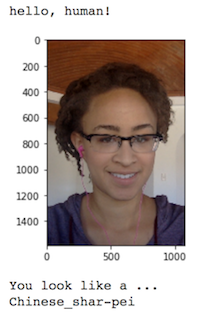
\includegraphics{images/sample_human_output.png}
\caption{Sample Human Output}
\end{figure}

\hypertarget{implementation-write-your-algorithm}{%
\subsubsection{(IMPLEMENTATION) Write your
Algorithm}\label{implementation-write-your-algorithm}}

    \begin{Verbatim}[commandchars=\\\{\}]
{\color{incolor}In [{\color{incolor}30}]:} \PY{c+c1}{\PYZsh{}\PYZsh{}\PYZsh{} TODO: Write your algorithm.}
         \PY{c+c1}{\PYZsh{}\PYZsh{}\PYZsh{} Feel free to use as many code cells as needed.}
         
         \PY{k}{def} \PY{n+nf}{run\PYZus{}app}\PY{p}{(}\PY{n}{img\PYZus{}path}\PY{p}{)}\PY{p}{:}
             
             \PY{n}{img} \PY{o}{=} \PY{n}{Image}\PY{o}{.}\PY{n}{open}\PY{p}{(}\PY{n}{img\PYZus{}path}\PY{p}{)}
             \PY{n}{plt}\PY{o}{.}\PY{n}{imshow}\PY{p}{(}\PY{n}{img}\PY{p}{)}
             \PY{n}{plt}\PY{o}{.}\PY{n}{show}\PY{p}{(}\PY{p}{)}
             
             \PY{c+c1}{\PYZsh{}\PYZsh{} handle cases for a human face, dog, and neither}
             \PY{k}{if} \PY{n}{dog\PYZus{}detector}\PY{p}{(}\PY{n}{img\PYZus{}path}\PY{p}{)} \PY{o+ow}{or} \PY{n}{face\PYZus{}detector}\PY{p}{(}\PY{n}{img\PYZus{}path}\PY{p}{)}\PY{p}{:}
                 \PY{n+nb}{print}\PY{p}{(}\PY{l+s+s2}{\PYZdq{}}\PY{l+s+s2}{You look like a ...}\PY{l+s+s2}{\PYZdq{}}\PY{p}{,} \PY{n}{predict\PYZus{}breed\PYZus{}transfer}\PY{p}{(}\PY{n}{img\PYZus{}path}\PY{p}{)}\PY{p}{)}
             \PY{k}{else}\PY{p}{:}
                 \PY{n+nb}{print}\PY{p}{(}\PY{l+s+s2}{\PYZdq{}}\PY{l+s+s2}{This does not look like a dog or human!}\PY{l+s+s2}{\PYZdq{}}\PY{p}{)}
\end{Verbatim}


    \begin{center}\rule{0.5\linewidth}{\linethickness}\end{center}

 \#\# Step 6: Test Your Algorithm

In this section, you will take your new algorithm for a spin! What kind
of dog does the algorithm think that \emph{you} look like? If you have a
dog, does it predict your dog's breed accurately? If you have a cat,
does it mistakenly think that your cat is a dog?

\hypertarget{implementation-test-your-algorithm-on-sample-images}{%
\subsubsection{(IMPLEMENTATION) Test Your Algorithm on Sample
Images!}\label{implementation-test-your-algorithm-on-sample-images}}

Test your algorithm at least six images on your computer. Feel free to
use any images you like. Use at least two human and two dog images.

\textbf{Question 6:} Is the output better than you expected :) ? Or
worse :( ? Provide at least three possible points of improvement for
your algorithm.

    \textbf{Answer:} I expected a bit better output, however, I did not
train my model extensively. I only run 20 epochs, which is a low number.
Accuracy would be gladly improved by more extensive training.

    \begin{Verbatim}[commandchars=\\\{\}]
{\color{incolor}In [{\color{incolor}33}]:} \PY{c+c1}{\PYZsh{}\PYZsh{} TODO: Execute your algorithm from Step 6 on}
         \PY{c+c1}{\PYZsh{}\PYZsh{} at least 6 images on your computer.}
         \PY{c+c1}{\PYZsh{}\PYZsh{} Feel free to use as many code cells as needed.}
         
         \PY{c+c1}{\PYZsh{}\PYZsh{} suggested code, below}
         \PY{k}{for} \PY{n}{file} \PY{o+ow}{in} \PY{n}{np}\PY{o}{.}\PY{n}{hstack}\PY{p}{(}\PY{p}{(}\PY{n}{human\PYZus{}files}\PY{p}{[}\PY{p}{:}\PY{l+m+mi}{3}\PY{p}{]}\PY{p}{,} \PY{n}{dog\PYZus{}files}\PY{p}{[}\PY{p}{:}\PY{l+m+mi}{3}\PY{p}{]}\PY{p}{)}\PY{p}{)}\PY{p}{:}
             \PY{n}{run\PYZus{}app}\PY{p}{(}\PY{n}{file}\PY{p}{)}
\end{Verbatim}


    \begin{center}
    \adjustimage{max size={0.9\linewidth}{0.9\paperheight}}{output_59_0.png}
    \end{center}
    { \hspace*{\fill} \\}
    
    \begin{Verbatim}[commandchars=\\\{\}]
You look like a {\ldots} Bearded collie

    \end{Verbatim}

    \begin{center}
    \adjustimage{max size={0.9\linewidth}{0.9\paperheight}}{output_59_2.png}
    \end{center}
    { \hspace*{\fill} \\}
    
    \begin{Verbatim}[commandchars=\\\{\}]
You look like a {\ldots} Bull terrier

    \end{Verbatim}

    \begin{center}
    \adjustimage{max size={0.9\linewidth}{0.9\paperheight}}{output_59_4.png}
    \end{center}
    { \hspace*{\fill} \\}
    
    \begin{Verbatim}[commandchars=\\\{\}]
This does not look like a dog or human!

    \end{Verbatim}

    \begin{center}
    \adjustimage{max size={0.9\linewidth}{0.9\paperheight}}{output_59_6.png}
    \end{center}
    { \hspace*{\fill} \\}
    
    \begin{Verbatim}[commandchars=\\\{\}]
You look like a {\ldots} Affenpinscher

    \end{Verbatim}

    \begin{center}
    \adjustimage{max size={0.9\linewidth}{0.9\paperheight}}{output_59_8.png}
    \end{center}
    { \hspace*{\fill} \\}
    
    \begin{Verbatim}[commandchars=\\\{\}]
You look like a {\ldots} Affenpinscher

    \end{Verbatim}

    \begin{center}
    \adjustimage{max size={0.9\linewidth}{0.9\paperheight}}{output_59_10.png}
    \end{center}
    { \hspace*{\fill} \\}
    
    \begin{Verbatim}[commandchars=\\\{\}]
You look like a {\ldots} Affenpinscher

    \end{Verbatim}


    % Add a bibliography block to the postdoc
    
    
    
    \end{document}
